%%%%%%%%%%%%%%%%%%%%%%%%%%%%%%%%%%%%%%%%%%%%%%%%%%%%%%%%%%%%%%%%%%%%%%%%%%%%%%%
\chapter{Usage}\label{ChapUsage}
Ash3d 


%%%%%%%%%%%%%%%%%%%%%%%%%%%%%%%%%%%%%%%%%%%%%%%%%%%%%%%%%%%
\section{Preliminary meta-data}\label{ChapUsageSecPrelimData}
Wind files\\
Volcano data\\
Airport/POI data

%%%%%%%%%%%%%%%%%%%%%%%%%%%%%%%%%%%%%%%%%%%%%%%%%%%%%%%%%%%
\section{Running Ash3d on the command-line}\label{ChapUsageSecCommandLine}
The Linux command-line provides a more versatile but less
user-friendly environment for running Ash3d simulations.
We do not offer support for installing or running Ash3d
on computers outside the USGS, but we are willing to work
with collaborators who wish to run Ash3d in a more advanced
environment than is possible through the web interface.
Below, we explain how to set up and run a simulation in a
Linux environment. Ash3d is in a state of continuing
development, and we recommend that potential users consult
the authors for updates before following these instructions.

\begin{figure}[htbp]
%\includegraphics[angle=90,scale=0.9]{asharrivaltimesairports_p1.pdf}
\parbox{15cm}{\caption{\label{FigAsh3dOutput}
Examples of model output}}
\end{figure}

\subsection{Model input using an ASCII input file}
The Ash3d executable reads from an ASCII input file that
supplies information on source parameters, output file types,
and other options. A file for a simulation at Redoubt volcano
is illustrated in Appendix \ref{ChapAppendAuxFiles}.
%All elements in blue are
%comments; actual input parameters are shown in black.
If these
files are viewed in a Linux text editor such as \texttt{vi} or
\texttt{gedit}
that converts syntax elements for a shell script into colors,
the same color scheme will be visible, allowing users to easily
discriminate comments from parameters. The input file is further
divided into blocks, delimited with lines of asterisks. Each of
these blocks is described below.

\paragraph{Block 1}: Model grid\\
The lines in this block primarily define the size, shape,
and location of the model domain.
\small
\begin{verbatim}
*******************************************************************************
Spurr                               # Volcano name
1 4 -107.0 50.0 50.0 50.0 6367.47   # Proj flags and params
-154.0 58.0                         # x, y of LL corner of grid (km, or deg.)
20.0 6.0                            # grid width and height (km, or deg.)
-152.251 61.299 2.309               # vent location         (km, or deg.)
0.25       0.25                     # DX, DY of grid cells  (km, or deg.)
0.5                                 # DZ of grid cells      (always km)
0.0     4.0                         # diffusion coefficient (m2/s), Suzuki constant
1                                   # neruptions, number of eruptions or pulses
*******************************************************************************
\end{verbatim}
\normalsize

Line 1 gives either the volcano name or the volcano’s Smithsonian ID.
If the number begins with 0 or 1, then the volcano database used is
the Catalog of Active Volcanoes of the World [Siebert et al., 2010].
If the number does not begin with 0 or 1, then the Volcanoes of the
World (VOTW) database is used
[Global Volcanism Program, 2013. Volcanoes of the World, v. 4.9.4 (17 Mar 2021).
Venzke, E (ed.). Smithsonian Institution.
Downloaded 13 Apr 2021. https://doi.org/10.5479/si.GVP.VOTW4-2013. ].
If the CAVW number is given, Ash3d looks up the eruption source
parameters (ESP) for this volcano in the ESP spreadsheet of
\cite{Mastin09a}. In the example file, the volcano name
is given.

Line 2 gives the projection parameters for this simulation.
Ash3d uses the \texttt{volcano-ash3d-projection} package to specify the
projection and to calculate any needed coordinate transformations.
Documentation for this package can be found at
\url{https://github.com/DOI-USGS/volcano-ash3d-projection}.
These parameters on Line 2 define the projection for the computational
grid and can be different than the projection used for the numerical
weather prediction (NWP) files. Some of
those NWP models, such as the NOAA National Center for Environmental
Prediction’s (NCEP) Global Forecast System (GFS) model, are run
on a spherical earth, hence the wind vectors are given in a 3-D
grid of longitude, latitude, at pressure levels. Other models, such
as NOAA’s North American Model are run using a grid that is
projected onto a planar coordinate system. After Ash3d reads
the NWP atmospheric data, it must know the type of projection in order
to find the portion of the NWP model grid that lies within the
Ash3d model domain.
Ash3d uses the MetReader library to read the atmospheric data and to
interpolate values from the NWP grid onto the computational grid used
by Ash3d. MetReader also projects the wind vectors onto the coordinate
system specified by this line.
The types of NWP model output that
Ash3d can read, and their projection parameters, are given in
Table \ref{tab:ProjOpt}.
The first two parameters on this line are \texttt{latlonflag} and
\texttt{projflag},
where:
\begin{itemize}
 \item \texttt{latlonflag} is an integer whose value is 0 if coordinate system is
projected, 1 if coordinates are in longitude and latitude
 \item \texttt{projflag} is an integer that indicates the projection type
\end{itemize}
Numbers that follow these two integer flags are the projection parameters
that are different for different map projections.
\small
\begin{table}[htbp]
\begin{center}
\begin{tabular}{| c | c | l | l |}
\hline
\texttt{latlonflag} & \texttt{projflag} & Description & Expected parameters\\
\hline
0 & 0 & Non-geographic Cartesian grid & N/A \\
0 & 1 & Polar Stereographic & $\lambda_0$ $\phi_0$ $k_0$ $R_e$ \\
0 & 2 & Albers Equal Area & $\lambda_0$ $\phi_0$ $\phi_1$ $\phi_2$ $R_e$ \\
0 & 3 & UTM & Not yet functional \\
0 & 4 & Lambert Conformal Conic & $\lambda_0$ $\phi_0$ $\phi_1$ $\phi_2$ $R_e$\\
0 & 5 & Mercator & $\lambda_0$ $\phi_0$ $R_e$\\
1 & N/A & Longitude/Latitude & N/A \\
\hline
\end{tabular}
\caption{\label{tab:ProjOpt}Ash3d projection options}
\end{center}
\end{table}
\normalsize
Below are some examples of
this input line. The comment in blue following the hash mark (\#) gives
the projection type.\\
\texttt{0 1 -135.0 90.0 0.933 6371.229 {\color{blue} \#Polar stereographic}}\\
Parameters 3-6 are
$\lambda_0$, the longitude of the projection point;
$\phi_0$, the latitude of the projection point;
$k_0$, the scale factor at the projection point;
and $R_e$, the Earth radius used in kilometers.\\
\texttt{0 4 -95. 25.0 25.0 25.0 6371.229 {\color{blue} \#Lambert Conformal Conic}}\\
Parameters 3-7 are
$\lambda_0$, the longitude of the projection origin;
$\phi_0$, the latitude of the projection origin;
$\phi_1$, the latitude of the first secant;
$\phi_2$, the latitude of the second secant;
and $R_e$, the Earth radius used.

Line 3 gives the x and y (or longitude and latitude if \texttt{latlonflag = 1})
values of the lower
left corner of the grid. These values must be in the same coordinate system
defined by the projection parameters on line 2.

Line 4 gives the model domain width and height, in degrees if longitude and latitude
are used, or kilometers if a projected coordinate system is used.
If longitude and latitude are used and if the width is given as 360$^{\circ}$,
then Ash3d uses a periodic grid.

Line 5 gives the vent location, also in the same units as the specified
coordinate system. This line may take either two or three values. The first
two values are required and correspond to the x and y (or longitude and
latitude) coordinates of the vent. A third, optional value gives to the
vent’s elevation in
kilometers. If no elevation is given, Ash3d assigns the volcano an elevation
equal to that of the topography at this location, or zero if topography is
not used in this model run. For the web interface, topography is not used.

Line 6 gives the horizontal grid spacing in the model, in kilometers if a
projected grid is used, or degrees if longitude/latitude are used. If the
width and height of the model domain are not an integral number of cell
distances, the location of the upper right corner of the model domain is
adjusted to be an integral number of cell distances from the lower left
corner.

Line 7 specifies the vertical grid structure to be used. If a number is
given, it is interpreted to be the constant $\Delta z$ for a regular vertical
grid spacing.
The units of this input parameter are always kilometers.
Alternatively, a text string can be given which specifies
different options for a variable spacing of the vertical grid. This text
string must be one of the following:
\begin{itemize}
\item \texttt{dz\_plin}: for piecewise linear
\item \texttt{dz\_clog}: for constant $\Delta z$ in $\log z$
\item \texttt{dz\_cust}: for custom
\end{itemize}
For each of these variable-$\Delta z$ cases, an additional line must be
provided in the input file immediately after Line 7. For \texttt{dz\_plin},
this line must start with the number of linear segments, followed by the
number of cells and $\Delta z$ in each segments
($n_{seg}$ $n_{z_1}$ $\Delta z_1$ $n_{z_2}$ $\Delta z_2$ $\cdots$ $n_{z_n}$ $\Delta z_n$).
For \texttt{dz\_clog}, the additional line just contains $z_{top}$ followed by
the number of cells in $z$.
For \texttt{dz\_cust}, the additional line must start with the vertical
number of cells $nz$, followed by a list of $nz$ values for
$\Delta z$.

Line 8 parameters specify the diffusion coefficient ($K$) and the
vertical distribution of mass in the column, respectively. The diffusion
coefficient is specified in $\mathrm{m^2/s}$ and is applied to both the
horizontal and vertical diffusivities. If $K$=0.0, Ash3d disables the
diffusion calculation. Note that unless Ash3d has been
compiled with the Crank-Nicolson scheme invoked (which requires the \texttt{lapack}
library), including diffusion can significantly increase the computation time
through the time-step constraints with explicit diffusion solvers.

The vertical distribution of mass may be specified either as a number, or as a
text string: \texttt{point}, \texttt{line},
\texttt{profile}, \texttt{umbrella}, and \texttt{umbrella\_air}.
These possibilities are illustrated in Figure \ref{FigVertMassDistFormat}. If the input is:

\begin{figure}[htbp]\vspace*{-5cm}\hspace*{-2cm}
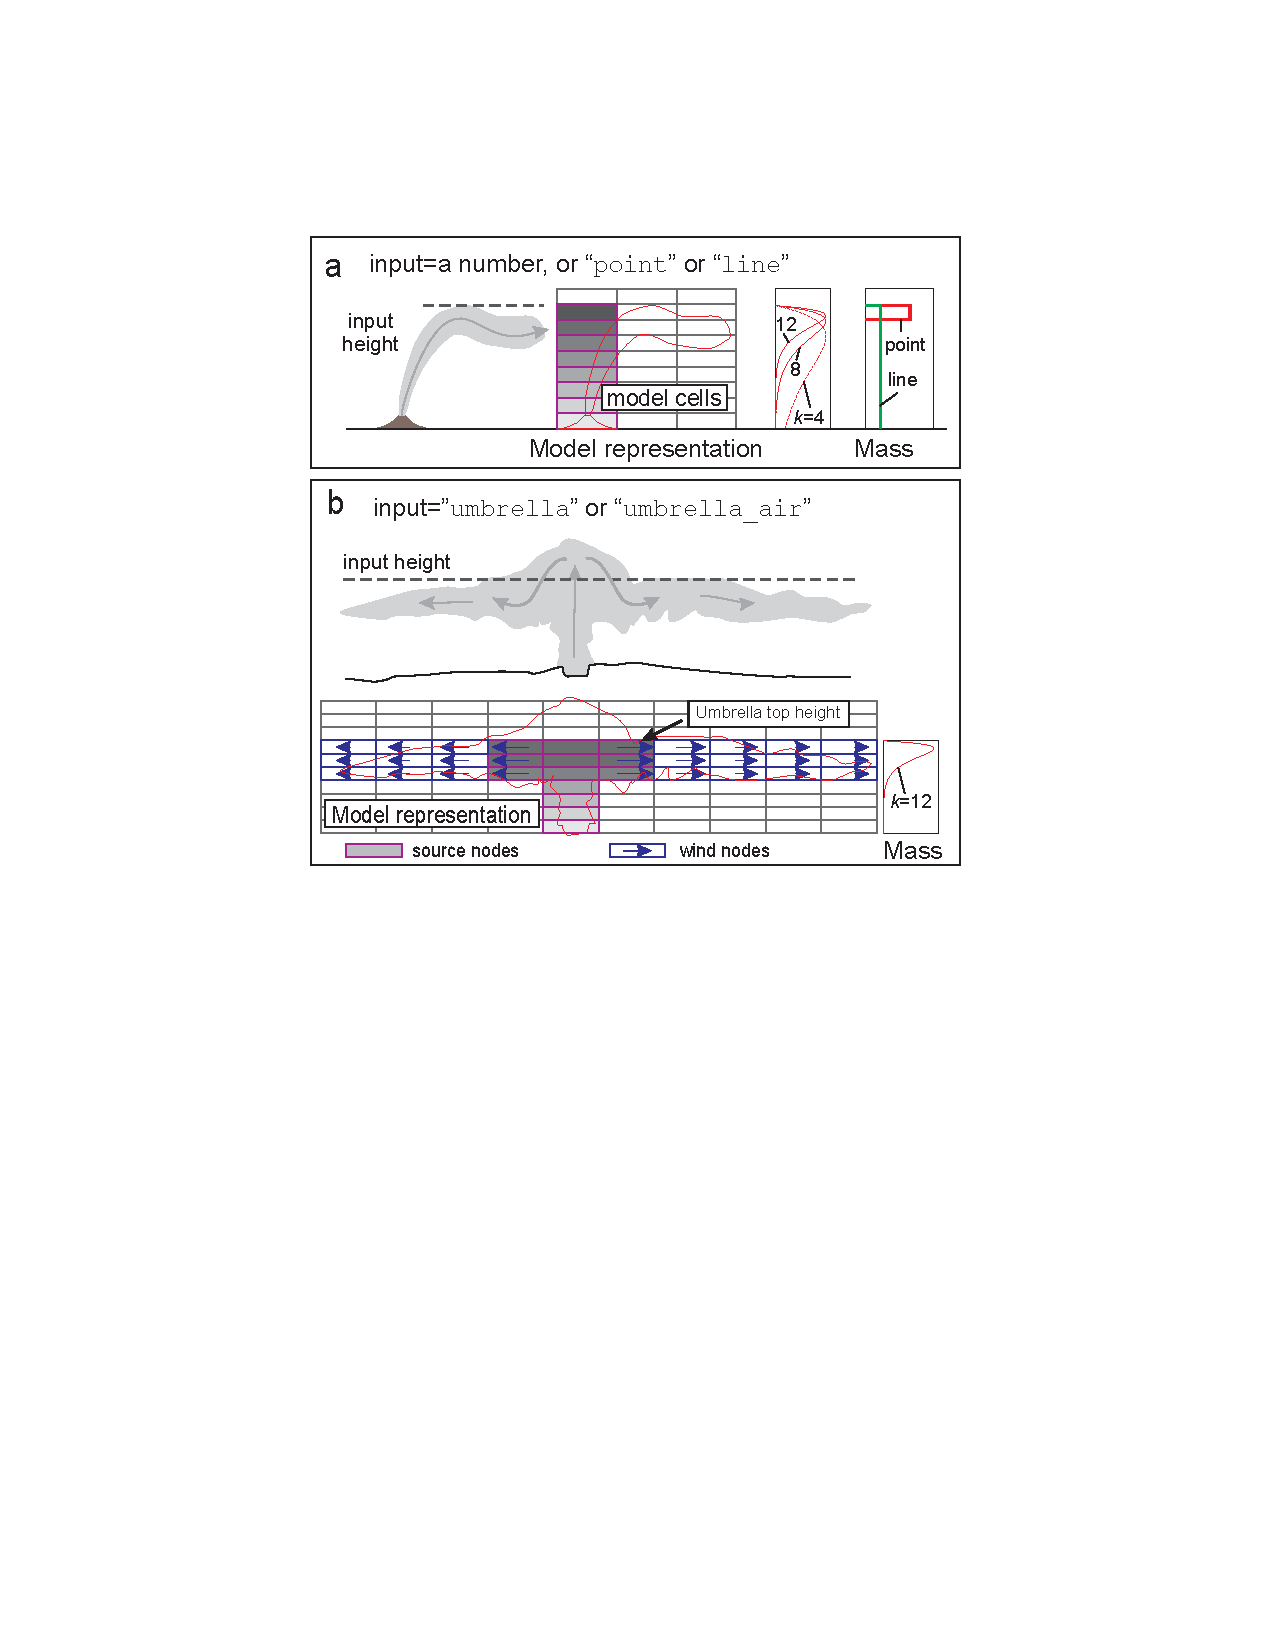
\includegraphics[angle=0,scale=0.8]{Figures/Scripts/VertMassDist.pdf}
\parbox{15cm}{\caption{\label{FigVertMassDistFormat}
Illustration of vertical mass distributions that can be specified in Ash3d, and
the association of these inputs with other aspects of model setup, such as plume
height and the configuration of source nodes.
}}
\end{figure}

\begin{itemize}
\item a number: it is assumed to be the Suzuki constant $k$ in Equation \ref{EqSuz}.
Mass distributions for different $k$ are illustrated in Figure \ref{FigVertMassDistFormat}a.
\item \texttt{point}: all mass is placed in a single cell at the
plume top (Figure \ref{FigVertMassDistFormat}a).
\item \texttt{line}: mass is distributed evenly from the vent
elevation (if provided) or from sea level (if vent elevation is not
provided) to the plume top (Figure \ref{FigVertMassDistFormat}a)
\item \texttt{profile}: each eruptive pulse line in Block 2 must be supplemented
by an additional line specifying the profile, as described below.
\item \texttt{umbrella} or \texttt{umbrella\_air}: the plume height in Block 2 is
interpreted as the height of the umbrella cloud (ash in the overshooting
top, above the umbrella cloud, is assumed to collapse gravitationally
back into the umbrella rather than being advected horizontally by winds at that
altitude). This source type is most appropriate for eruptions of VEI=6 and larger,
and may be appropriate for some VEI 4 or 5 eruptions \cite{Mastin20}. Source
nodes for these cases consist of a column of nodes extending from the vent
elevation (if provided) to 75\% of the umbrella top height, or from sea level
(if vent elevation is not provided) to 75\% of the umbrella top height. From
75\% to 100\% of the umbrella top height, source nodes consist of a matrix $3 \times 3$
in plan view (Figure \ref{FigVertMassDistFormat}b). Within the height range of
the $3 \times 3$ matrix, from the vent outward to the edge of the expanding
umbrella cloud, radial wind vectors are added to the ambient wind field.
The magnitude of the radial wind vectors is calculated using corrected
Equations (2) and (3) of \cite{Costa13}, and is proportional to the mass
eruption rate.
The only difference between \texttt{umbrella} and \texttt{umbrella\_air} is that the
latter is used only for simulations of airborne ash, where a single grain
size is used, and the volume of ash is assume to equal 5\% of the total
erupted volume. Only one eruptive pulse may be specified when the umbrella
source is used.
%VelMod\_umb 1=Eq. 3; 2=Eq. 4
%k_entrainment_umb, lambda_umb, N_BV_umb, SuzK_umb
%
\item neither a number nor one of the above types: Ash3d assumes this
source type is a user-specified custom source type.
These are described in detail in section \ref{SecOptionalModulesUserCust}
\end{itemize}

Line 9 gives the number of eruptions or eruptive pulses in the simulation.
The eruptions or eruptive pulses may be either contiguous or non-contiguous
in time. Their duration should not be shorter than the average time step
in the model (about a minute).

\paragraph{Block 2}: Eruptive pulses\\
For the standard source types (\texttt{suzuki}, \texttt{point}, \texttt{line},
\texttt{umbrella}, or \texttt{umbrella\_air}),
the number of lines in this block equals the number of eruptions or eruptive
pulses specified in Line 9 of Block 1.
A line of input for these types contains three integers followed by four
real numbers, for example:
\small
\begin{verbatim}
*******************************************************************************
1992 08 19   1.0   3.5     13.7   0.014
*******************************************************************************
\end{verbatim}
\normalsize

The first four numbers represent the year, month, day and hour (UTC) of the
start of the eruption. The following three numbers represent the eruption
duration in hours, the plume height in kilometers above sea level, and the
erupted volume in cubic kilometers dense-rock equivalent (DRE). Ash3d converts
the erupted volume to a mass assuming a magma density of 2500 $\mathrm{kg/m^3}$.
This can be changed at run-time is desired (See Section \ref{}).
If the year is zero as in the example input file, the model is run in forecast
mode where the hour is interpreted as the number of hours after the start time
of the wind files. In addition, if the duration, plume height, or erupted volume
is negative, it is replaced with the default ESP value for that volcano from the
spreadsheet of \cite{Mastin09b}.

If the source type is \texttt{profile}, then the eruption lines are read as
three integers, five real numbers, and an integer where
two numbers are the $\Delta z$ and number of $z$-points defining
the profile.  This type of source type must have a line following with the list
of fractional values for each of the $\Delta z$ segments (should total unity).
An example of this type is given below.
\small
\begin{verbatim}
*******************************************************************************
1992 08 19   1.0   3.5  0.1  13.7   0.5 14
0.0 0.1 0.1 0.1 0.1 0.2 0.2 0.0 0.0 0.0 0.05 0.05 0.1 0.0
*******************************************************************************
\end{verbatim}
\normalsize

\begin{figure}[htbp]
%\includegraphics[angle=90,scale=0.9]{asharrivaltimesairports_p1.pdf}
\parbox{15cm}{\caption{\label{FigSourceOptions}
Example of source term options}}
\end{figure}
If the source type is not recognized, Ash3d just reads the first line of this
block which must have at a minimum three integers for the year, month and day,
followed by three real values for the hour, duration and height.  There may
be more values on the eruption source line and potentially additional lines to
read for the custom sources, but this is parsed later after the remaining blocks
are read.

\paragraph{Block 3}: Wind files and simulation time\\
Line 1 of Block 3 gives at least two integers, \texttt{iwind} and \texttt{iwindformat}.
The first number (\texttt{iwind}) specifies the structure of the windfiles and can
have the following values:
1=1-D wind sounding(s),
2=3-D gridded ASCII files,
3=a single NWP file (all variable data for all steps in one file),
4=multiple NWP files (all variable data for one step in individual files),
5=non-standard files that require hard-wired paths.
%\begin{center}
%\begin{tabular}{| c | l |}
%\hline
%\texttt{iwind} & Description \\
%\hline
%1& 1-D wind sounding(s) \\
%2& 3-D gridded ASCII files \\
%3& a single NWP file (all variable data for all steps in one file) \\
%4& multiple NWP files (all variable data for one step in individual files)\\
%5& non-standard files that require hard-wired paths \\
%\hline
%\end{tabular}
%\end{center}

The distinction between \texttt{iwind}=3 and \texttt{iwind}=4 has been
relaxed and these are now interchangeable.
Ash3d attempts to read two more integer values on Line 1
of this block: a grid ID, and a format code. The grid code is the NCEP grid
ID described at \url{http://www.nco.ncep.noaa.gov/pmb/docs/on388/tableb.html}
and the format code must be either 1 (ASCII), 2 (NetCDF), or 3 (GRIB v1 or v2).
If these values are not provided, the grid code is assigned if known from the
NWP product given by \texttt{iwindformat} and the data format code is assumed to
be 2=NetCDF. The combinations of \texttt{iwind} and \texttt{iwindformat} are shown in
Table \ref{tab:MetOptions}.

\small
\begin{table}[htbp]
\begin{center}
\begin{tabular}{| c | c| c | c | l |}
\hline
\texttt{iwind} & \texttt{iwindformat} & \texttt{grid} & \texttt{data} &Description \\
\hline
1& & & & 1-D wind sounding(s) \\
\hline
 &1&n&1& User-specified \\
 &2&n&1& global radiosonde data \\
\hline
2& & & &3-D gridded ASCII files \\
 & & & &Not implemented/deprecated\\
\hline
3& & & &one NWP file for all data\\
4& & & &one NWP file per time step\\
\hline
 & 0& &2&User-defined via template\\
 & 3&221&2/3&North American Regional Reanalysis NARR\\
 & 4&221&2/3&NAM Regional North America\\
 & 5&216&2/3&NAM Regional Alaska\\
 & 6&104&2/3&NAM N. Hemisphere\\
 & 7&212&2/3&NAM Regional CONUS\\
 & 8&218&2/3&NAM Regional CONUS\\
 & 9&227&2/3&NAM Regional CONUS\\
 &10&242&2/3&NAM Regional Alaska\\
 &11&196&2/3&NAM Regional Hawaii\\
 &12&198&2/3&NAM Regional Alaska\\
 &13& 91&2/3&NAM Regional Alaska\\
 &14&   &2/3&NAM Regional CONUS \\
 &20&  4&2/3&GFS\\
 &21&  3&2/3&GFS\\
 &22&193&2/3&GFS\\
 &23&  2&2/3&NCEP-DOE Reanalysis 2\\
 &24&   &2/3&NASA-MERRA-2 Reanalysis\\
 &25&  2&2/3&NCEP/NCAR Reanalysis 1\\
 &28&170&2/3&ECMWF ERA-Interim Reanalysis\\
 &32&   &2/3&Air Force Weather Agency subcenter = 0\\
 &33&   &2/3&CCSM3.0 Community Atmosphere Model\\
 &40&   &2/3&NASA GEOS-5 Cp\\
 &41&   &2/3&NASA GEOS-5 Np\\
 &50&   &2/3&WRF - output\\
\hline
5& & & &files that require hard-wired paths \\
\hline
 &25&  2&2/3&NCEP/NCAR Reanalysis 1\\
 &26& 45&2/3&JRA-55\\
 &27&  2&2/3&NOAA-CIRES 20th Century Reanalysis\\
 &29&   &2/3&ECMWF ERA5 Reanalysis\\
 &30&   &2/3&ECMWF ERA-20C Reanalysis\\
\hline
\end{tabular}
\caption{\label{tab:MetOptions}Ash3d options for wind data}
\end{center}
\end{table}
\normalsize

If \texttt{iwind}=1, Ash3d reads from one or more ASCII files of a 1-D wind sounding.
%format shown in Table \ref{}.
This option can be used if no numerical weather prediction
data are available or if data from radiosonde measurements is deemed more
reliable than NWP model results.
If \texttt{iwindformat}=1, then Ash3d expects the user-provided files to have a format
of 3 header lines, followed by three or more columns of data. The format specification
is documents in the MetReader User's Guide, but also outlined in the
Appendix \ref{ChapAppendAtmosDataFormat1d}.

If \texttt{iwindformat}=2, then Ash3d expects the 1-D profile to be from the global
radiosonde data available from \url{https://ruc.noaa.gov/raobs/} or from
\url{http://weather.uwyo.edu}. Details on the particular formats Ash3d is able to
read is described in Appendix \ref{ChapAppendAtmosDataFormat1d}.

Since there is no grid for these data, \texttt{igrid}, if provided, is interpreted to
be the number of stations with 1-D data. The number of windfiles must be an even
multiple of \texttt{igrid}.

When \texttt{iwind}=2, Ash3d reads a 3-D atmospheric fields in ASCII format that is converted from
NetCDF format using a Java script that was originally written before Ash3d was
modified to read NetCDF files directly. This option is no longer used.
\texttt{iwind}= 3 or 4 indicates that the atmospheric files contain 3-D time-series
data. Originally, \texttt{iwind}=3 was used for indicating that all data were stored in
a single file with multiple time steps, and \texttt{iwind}=4 was for multiple NetCDF files,
each for one time step. This distinction is deprecated as currently, all data
files provided with \texttt{iwind}= 3 or 4 are evaluated for the time steps available.
This then can accommodate the occasional NWP products that provide data in a
multiple-file, multiple-time-step format.

For some reanalysis products that do not store data in the above formats, such as
the products that store a month or a year of data for only one variable in a single
file (e.g. NCEP NCAR 50-year reanalysis, \texttt{iwind}=5 can be used. For these cases,
Ash3d expects the NWP files to have specific filenames and to be stored in a
specific directory structure. Details for these products are described in the MetReader
documentation and summarized in Chapter \ref{ChapAppendAtmosDataFormat1d}.

%The two options were
%created to accommodate different posting conventions for different kinds of wind
%files. For example, Global Forecast System output files posted at Unidata
%(\url{http://unidata.ucar.edu}) for current and forecast conditions include a separate
%file for every three-hour time step. Alaska 11km North American Model forecasts
%posted at Unidata are given as a single file for multiple time steps.
%The second parameter, \texttt{iwindformat}, indicates the type of NWP file to be read. The
%values of \texttt{iwindformat} for each NWP file type are listed in Table \ref{}.
Line 2 gives the integer \texttt{iHeightHandler}, which indicates how Ash3d should respond
if it finds that the plume height exceeds the highest level in the NWP model.
Numerical weather prediction models give 3-D atmospheric fields with the vertical coordinate
in pressure levels. For the GFS 0.5 degree model, the lowest pressure level is
$\sim 40 \,\mathrm{kPa}$,
which corresponds to about $50 \mathrm{km}$ altitude.
The atmospheric conditions at higher altitude is
unknown from these models. If the input plume height is higher than the highest
altitude in the NWP model, Ash3d responds in one of the following ways: if
\texttt{iHeightHandler}=1, Ash3d execution stops and writes an error message to standard output
and the log file.
If \texttt{iHeightHandler}=2, Ash3d continues execution and uses the wind vectors in the
top-most pressure level in all lower pressure levels. Temperature is calculated for these
higher altitudes using the US Standard Atmosphere. Ash3d also writes a warning
message to standard output and to the log file.

Line 3 gives the simulation time in hours. The simulation time is assumed to start
at the time of the first eruption or eruptive pulse. Ash3d checks the time duration
of the atmospheric files to ensure that the entire simulation time is contained within
the scope of provided files.

Line 4 is a ``yes'' or ``no'' parameter that specifies whether to stop computation
when 99\% of the erupted mass has left the domain either through deposition or
advecting out the boundaries. Setting this parameter to ``yes''
allows for faster execution if users are primarily interested in simulating
deposition. If simulating ash-cloud transport is of primary interest, users may
prefer to set this parameter to ``no''.

Line 5 specifies \texttt{nwindfiles}, the number of atmospheric files to be read.
%If more than one file is to be read, the parameter iwind in Block 3, line 1, must equal 4.
%Ash3d assumes in that case that each wind file contains a single time slice.
Ash3d examines the time stamp of all the steps of all the atmospheric files to ensure
that the start time and end time of the simulation are within the scope of the
provided files.

\paragraph{Block 4}: Output options\\
Most lines in this block specify types of output options that can be written at
specific output steps.
Lines 1-15 require ``yes'' or ``no'' to indicate whether a particular type of output
should be written. These types of output are listed in Table \ref{tab:OutputOptions}
along with the names of files written out.
\small
\begin{table}[htbp]
\begin{center}
\begin{tabular}{|r|l|l|l|l|}
\hline
Line & Output type&Variable&units & File names\\
\hline
 1&ASCII &final deposit thickness&$\mathrm{mm}$&DepositFile\_\_\_\_\_final.dat\\
 2&KML&final deposit thickness&$\mathrm{mm}$&deposit\_thickness\_mm.kml\\
  & & &$\mathrm{inches}$&deposit\_thickness\_inches.kml\\
 3&ASCII &transient deposit&$\mathrm{mm}$&Deposit\_xxx.xxhrs.dat\\
 4&KML&transient deposit&$\mathrm{mm}$&deposit\_thickness\_mm.kml\\
  & & &$\mathrm{inches}$&deposit\_thickness\_inches.kml\\
 5&ASCII &ash-cloud concentration&$\mathrm{mg/m^3}$&CloudConcentration\_xxx.xxhrs.dat\\
 6&KML& ash-cloud concentration&$\mathrm{mg/m^3}$&CloudConcentration.kml\\
 7&ASCII&ash-cloud height&$\mathrm{km}$&CloudHeight\_xxx.xxhrs.dat\\
 8&KML&ash-cloud height&$\mathrm{km}$&CloudHeight.kml\\
 9&ASCII&transient ash-cloud load&$\mathrm{T/km^2}$&CloudLoad\_xxx.xxhrs.dat\\
10&KML&transient ash-cloud load&$\mathrm{T/km^2}$&CloudLoad.kml\\
11&ASCII&deposit arrival times&$\mathrm{hours}$&DepositArrivalTime.dat\\
12&KML&deposit arrival times&$\mathrm{hours}$&ashfall\_arrivaltimes\_hours.kml\\
13&ASCII&cloud arrival times&$\mathrm{hours}$&CloudArrivalTime.dat\\
14&KML&cloud arrival times&$\mathrm{hours}$&cloud\_arrivaltimes\_hours.kml\\
15&&consolidated output file&&specified in input file\\
\hline
\end{tabular}
\caption{\label{tab:OutputOptions}Block 4 options for output data}
\end{center}
\end{table}
\normalsize
The ESRI\textsuperscript{\tiny\textregistered} ASCII files noted in Table \ref{tab:OutputOptions}
are ASCII files written in a format that
can be directly imported into Arc\textsuperscript{\tiny\textregistered}
GIS products for display.
These files can also be easily converted to a format suitable for plotting with
Generic Mapping Tools (GMT) with the command:
\begin{verbatim}
gmt grdconvert DepositFile___final.dat=ef out.grd
\end{verbatim}
These files contain a six-line
header followed by a 2-D matrix containing values of, for example deposit thickness.
The header looks like:
\small
\begin{verbatim}
NCOLS 140
NROWS 140
XLLCORNER -2616390.
YLLCORNER 1742330.
CELLSIZE 5000.000 5000.000
NODATA_VALUE -9999.
\end{verbatim}
\normalsize

The parameters \texttt{XLLCORNER} and \texttt{YLLCORNER} give the coordinates
of the lower-left
corner of the model domain in meters (if it is a projected grid) or degrees (if
the grid is latitude/longitude). The cell size is in the same units as the corner
coordinates. 
Ash3d can generate grids whose x and y spacing are unequal, and this is
typically the case for simulations generated using the web interface. But Arc
products require the x and y spacing to be equal.
%Note: If you plan to import
%the ESRI\textsuperscript{\tiny\textregistered} ASCII files into
%Arc products, make sure to specify equal x and y cellsize
%on Line 6 of Block 1.
The KML files are written using Keyhole Markup Language and can be opened by
Google Earth\textsuperscript{\tiny\textregistered} or other virtual globe
software. The KML files can be zipped using the
following Linux command, which reduces file size by about 90-95\% and creates a
KMZ file that can also be opened in Google Earth:
\texttt{zip -r CloudLoad.kmz CloudLoad.kml}

The consolidated output file option specified in Line 15 of Table \ref{tab:OutputOptions}
serves several purposes. It is designed to store the store the full ash concentration
for each grain-size bin
of all cells at specified time steps in a format specified in Line 16. Current options
for this output format is \texttt{ascii}, \texttt{binary}, or \texttt{netcdf}.
If \texttt{netcdf}
is specified, this output file can serve as a restart file, allowing a failed or
suspended job to continue from the last output step. The NetCDF file contains
the full contents of the input file used to run the job to facilitate its
role as a restart file.
The NetCDF file also contains the various output variables that can be selected
in Lines 1-14 above. These include the following 2-D variables listed in
Table \ref{tab:OutputProducts}.

\small
\begin{table}[htbp]
\begin{center}
\begin{tabular}{|r|l|l|}
\hline
Variable Name                & Dimensions & units\\
\hline
\texttt{area}                & x,y        & $\mathrm{km^2}$   \\
\texttt{depothick}           & x,y,t      & $\mathrm{mm}$     \\
\texttt{depothickFin}        & x,y        & $\mathrm{mm}$     \\
\texttt{depotime}            & x,y        & $\mathrm{hours}$  \\
\texttt{ash\_arrival\_time}  & x,y        & $\mathrm{hours}$  \\
\texttt{ashcon\_max}         & x,y,t      & $\mathrm{mg/m^3}$ \\
\texttt{cloud\_height}       & x,y,t      & $\mathrm{km}$     \\
\texttt{cloud\_load}         & x,y,t      & $\mathrm{T/km^3}$ \\
\texttt{radar\_reflectivity} & x,y,z,t    & $\mathrm{dB}$     \\
\texttt{cloud\_bottom}       & x,y,t      & $\mathrm{km}$     \\
\texttt{depocon}             & x,y,gs,t   & $\mathrm{kg/m^2}$ \\
\texttt{ashcon}              & x,y,z,gs,t & $\mathrm{kg/km^3}$\\
\hline
\end{tabular}
\caption{\label{tab:OutputProduct}Output Products}
\end{center}
\end{table}
\normalsize

Optionally, an additional integer specifier can be included on
Line 15 to indicate if this consolidated output file should only contain the
2-D variables, which dramatically reduces the size of the output file, at the
expense of losing restart capabilities.
If this specifier is either absent or is 1, then the 3-D concentrations are written.
If it is 2, then only the 2-D output products are written.

Specifying \texttt{netcdf} in Line 16 provides the most general output product for post
processing. If Line 16 contains \texttt{ascii}, then data are written in ASCII format
to files names \texttt{3d\_tephra\_fall\_xxx.dat} where \texttt{xxx} is the output hour marker.
The output data are in column format in the following order: x (or lon), y (or lat), z,
total concentration (in $\mathrm{kg/km^3}$).
If \texttt{binary} is specified, then then total ash concentration is written to the files
\texttt{3d\_tephra\_fall\_xxx.raw} where \texttt{xxx} is the output hour marker.
Similarly, the deposit thickness is written to the files \texttt{2d\_tephra\_depo\_xxx.raw}.
The following
code sections shows how the data are written:
\begin{verbatim}
open(unit=20,file='3d_tephra_fall_'//cio//'.raw', &
     status='replace', &
     access='direct',recl=4*nxmax*nymax*nzmax)
write(20,rec=1)(((ashcon(i,j,k),i=1,nxmax),j=1,nymax),k=1,nzmax)
close(20)
open(unit=21,file='2d_tephra_depo_'//cio//'.raw', &
     status='replace', &
     access='direct',recl=4*nxmax*nymax)
write(21,rec=1)((DepositThickness(i,j),i=1,nxmax),j=1,nymax)
close(21)
\end{verbatim}
To read these files, you will need to know the values for \texttt{nxmax},
\texttt{nymax}, and \texttt{nzmax}. Although the default precision for
calculations in Ash3d is \texttt{real*8}, the default output precision is
\texttt{real*4} in order to reduce output file size. This can be changed, if desired
by editing the code in module \texttt{precis\_param} to set the internal
precision (\texttt{ip}) and the output precision (\texttt{op}).
See \ref{ChapSoftwareStructure}
for more details on editing these and other compile-time parameters.

The 3-D ash concentration file specified in Line 15 of Table \ref{tab:OutputOptions}
contains the full
3-D distribution of each grain size in the model domain at specified times.
The following lines complete this block of input:

Line 17 gives \texttt{nWriteTimes}, the number of times data are to be written out to the
files above. Data may be written out at uneven intervals (e.g. 0.2, 3, 3.4, and
12 hours after the eruption start) or at even intervals (e.g. every two hours,
starting 2 hours after the eruption start).

Line 18 gives the times at which output is written:
If \texttt{nWriteTimes}$>0$, Line 18 should contain \texttt{nWriteTimes}
numbers, in increasing order,
which specify the times in hours after the start of the eruption at which the above
data are to be written.
If \texttt{nWriteTimes}$=-1$, Line 18 should contain a single number indicating the time
interval in hours between write times.

\paragraph{Block 5}: Input wind files\\
This block should contain a number of lines equal to \texttt{nWindFiles} (Block 3, Line 5).
For the case of \texttt{iwind}$=5$, \texttt{nWindFiles} should be 1 and Block 5 Line 1
should be the path to the top-level directory of that product. For example, for the
NCEP $2.5^{\circ}$ Reanalysis files stored as:
\begin{verbatim}
/data/WindFiles/NCEP
|-- 2016
|   |-- air.2016.nc
|   |-- hgt.2016.nc
|   |-- omega.2016.nc
|   |-- uwnd.2016.nc
|   `-- vwnd.2016.nc
|-- 2017
    |-- air.2017.nc
    |-- hgt.2017.nc
    |-- omega.2017.nc
    |-- uwnd.2017.nc
    `-- vwnd.2017.nc
\end{verbatim}
only \texttt{/data/WindFiles/NCEP} should be given on Line 1.
Unless \texttt{iwindformat} (Block 3, Line 1) is 1 or 2, these files should be in
either NetCDF or GRIB
format and should consist of output from one of the model types listed in
Table \ref{tab:MetOptions}.
Each line gives the file name and path. In the example file, Ash3d reads a single
wind file named \texttt{latest.nc}, located in the subdirectory \texttt{Wind\_nc}.
Ash3d opens this
file and does a preliminary read to ensure that it covers the time period and
geographic region specified in input.

\paragraph{Block 6}: Arrival times at airports\\
The input lines in this block specify whether arrival times and other information
at specific locations are to be written to output. Normally, Ash3d reads from a
text input file containing the latitude and longitude (or x and y locations) of
a list of points. For the web interface, this is a global list of airports, but
when hand-editing the ASCII input file, other lists, such as sample locations, may
also be specified. Ash3d can then generate either text or KML files listing the
subset of these locations where ash was deposited or where the cloud passed overhead.
Ash3d can also write out the grain-size distribution of points at those locations.
All but line 4 require ``yes'' or ``no'' parameters.

Line 1 indicates whether to write out ash arrival times at these locations to an
ASCII file. If ``yes'' is given, an output file is generated called
\texttt{ash\_arrivaltimes\_airports.txt}
in the format shown in Figure \ref{FigAshArrivTimeFormat}.

\begin{figure}[htbp]\vspace*{-5cm}\hspace*{-2cm}
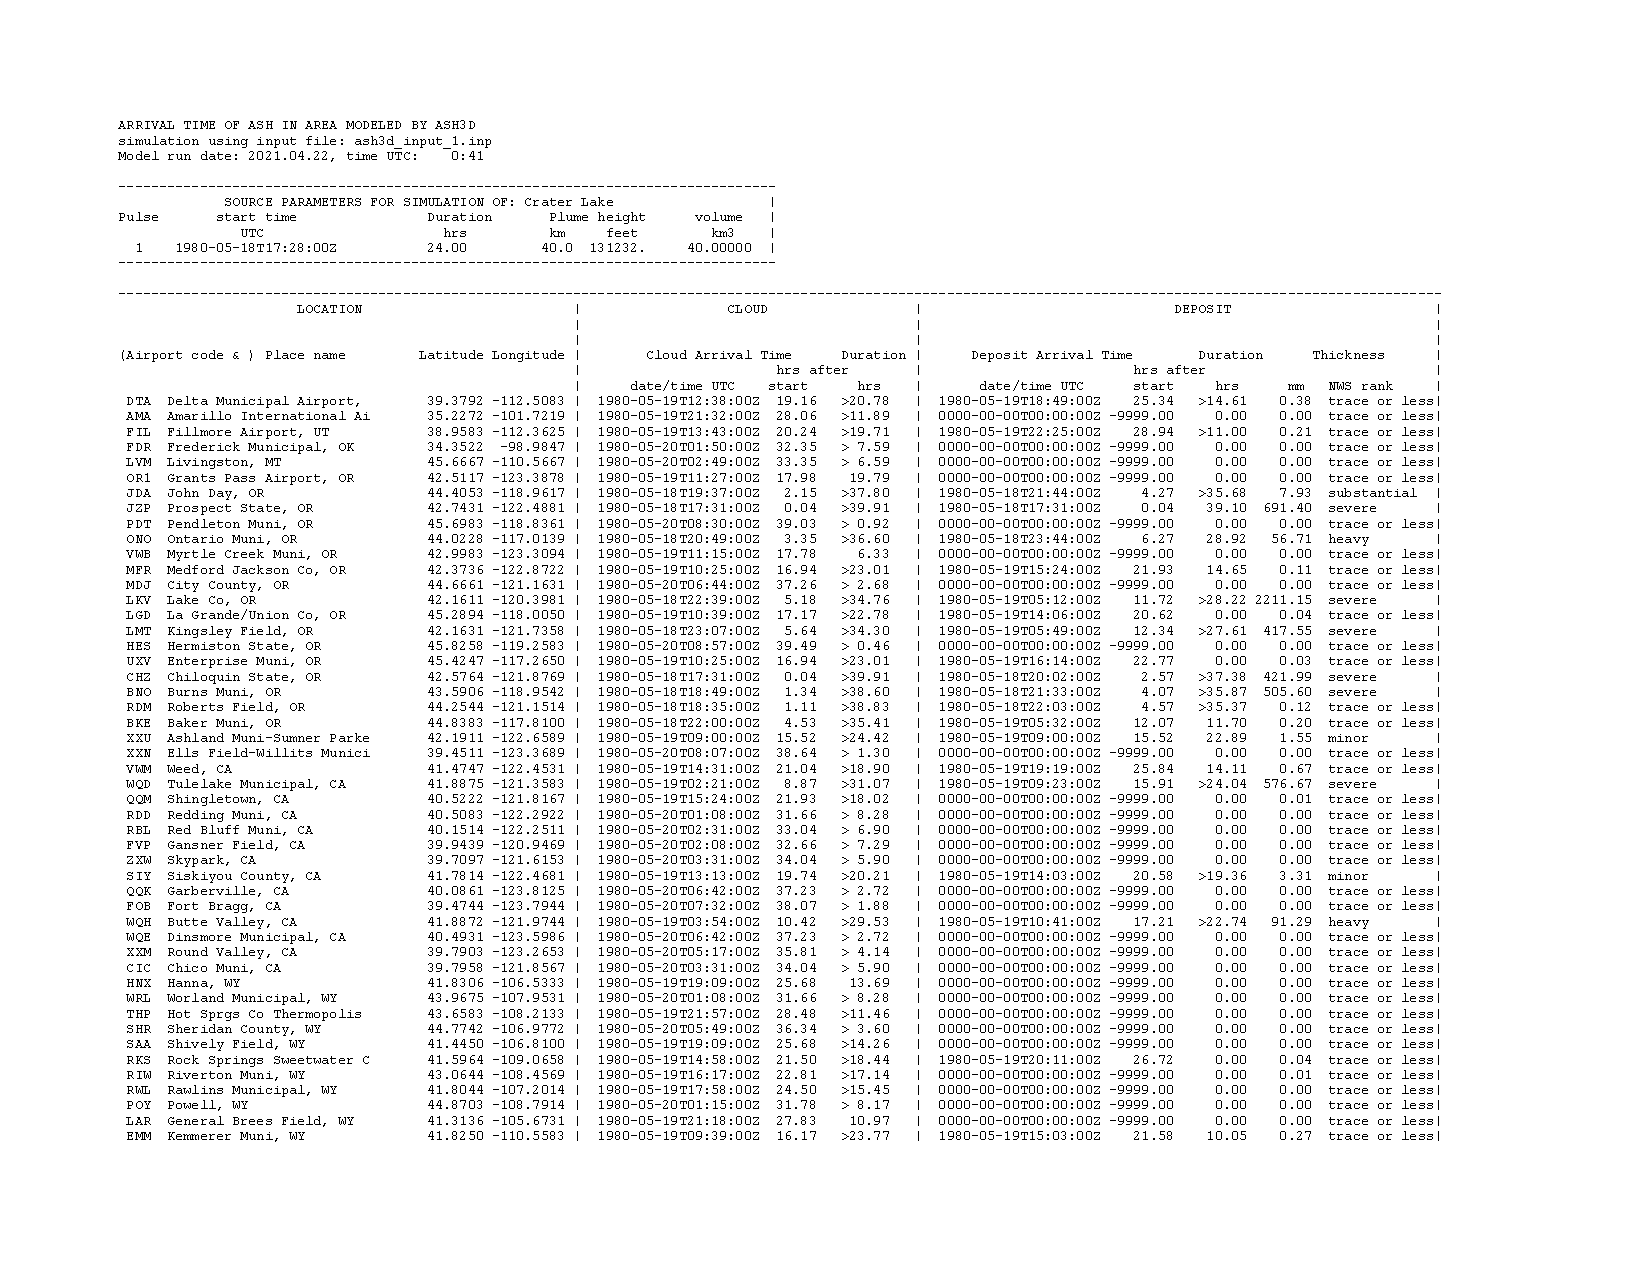
\includegraphics[angle=90,scale=0.9]{Figures/Chap_Usage_asharrivaltimesairports_p1.pdf}
\parbox{15cm}{\caption{\label{FigAshArrivTimeFormat}
Example of output file \texttt{ash\_arrivaltimes\_airports.txt}
}}
\end{figure}

Line 2 indicates whether the ASCII output file should give a grain-size distribution
of the tephra deposit at each location.

Line 3 indicates whether to write out a KML file showing the locations that will be
impacted by ash. If ``yes'' is given, a file named
\texttt{ash\_arrivaltimes\_airports.kml} is generated
that plots each impacted location as a red placemarks as shown in
Figure \ref{FigAsh3dOutput}.
Additionally, files for each impacted airport are generated that contain the data
for the ash accumulation as a function of time. These files are named
\texttt{depTS\_xxxx.dat} (where \texttt{xxxx} is the airport number in order of
time of ash arrival) and have two columns containing hour and ashfall thickness
in $\mathrm{mm}$. Additionally, a gnuplot script is written for each of these
airport locations so that time-series plots of ashfall accumulation can be embedded
in the KML files in post-processing.

Line 4 gives the name and path of the file containing airports or other locations
of interest. The format of this file must contain four columns with the location
information (latitude, longitude, x, y), followed by the 3-character IATA airport
code, then a 42-character descriptive string such as location. While the IATA
code is currently not used in any output products, the descriptive
string is use in ash arrival output products. An example of the expected format
for the airport file is given below.
\small
\begin{verbatim}
#   Latitude   Longitude           x           y  Code Location
    41.60833   -88.09417     0.00000     0.00000  II2  Lewis University Airport, IL
    34.68861   -85.29056     0.00000     0.00000  GA1  Barwick Lafayette Airport, GA
    58.36528  -152.69667     0.00000     0.00000  A33  Hidden Lake, AK
\end{verbatim}
\normalsize
In this case, airports with latitude and longitudes are given, but the x and y
columns are filled with 0.0 as a place-holder. If the computational grid is
Lon/Lat, then these airport coordinates will be used. If the computational 
grid is projected, then the x and y columns can be filled with the appropriate
values for the coordinate system used. Alternatively, the internal projection routines
can be used to generate the x and y values from the latitude and longitude columns.
This would over-write any values read in from the x and y columns of the file.
To specify that Ash3d should calculate the projected coordinates, Line 5 of
this block can be set to ``yes''. Ash3d would then convert the latitude and longitude
to the projected system specified in Block 1, Line 2. If this Line is ``no'' and 
if the computational grid is projected, then the x and y columns of the airport
file are used and the latitude and longitude columns are ignored.

Included with Ash3d is an internal list of 6117 global airports with IATA codes,
locations, and coordinates. By default, this is a filled variable at compile-time,
but optionally can be read at run-time from the
file \texttt{/opt/USGS/Ash3d/share/GlobalAirports\_ewert.txt}. If Line 4 of this
block is empty, or has the word ``internal'', then this built in list of global
airports is used. If an airport file name is provided, then this internal list
is replaced. Alternatively, if the first character of the file name provided is
`+', then the contents of the file are appended to the internal global list. For
example, if the block had the following form:
\small
\begin{verbatim}
****************** BLOCK 6 ***************************************************
yes              # Write out ash arrival times at airports to ASCII FILE?
no               # Write out grain-size distribution to ASCII airport file?
yes              # Write out ash arrival times to kml file?
+PointOfInt.txt  # Name of file containing aiport/POI locations
yes              # Have libprojection calculate projected coordinates?
*******************************************************************************
\end{verbatim}
\normalsize
then the global airport list would be extended by the contents of PointOfInterest.txt
with the x and y columns ignored in favor of the longitude and latitude or
internally projected mappings. The maximum number of airports is currently set
to 10,000.

\paragraph{Block 7}: Grain size groups\\
Ash3d can run an unlimited number of grain sizes, although the required run time
increases roughly in proportion to the number of grain sizes. To reduce model run
time, Ash3d stops calculations for individual grain sizes once they have left the
simulation domain, either advected out the sides or deposited. A grain size bin is
flagged as having left the simulation domain when $1 \, \mathrm{g}$ or less remains of
that grain size bin throughout the model domain.
When simulating ash clouds, one very small grain size ($0.01 \, \mathrm{mm}$ for
example) with a
very low settling velocity, is frequently adequate to display general cloud movement.
When simulating deposits, it is best to use at least a half dozen grain sizes: fewer
grain sizes tend to produce secondary thickness maxima as an artifact
\cite{Mastin12}.

Line 1 of Block 7 consists first of an integer giving the number of size bins
(\texttt{nsize}).
Optionally, a second integer can be provided which specifies the fall model to be used
(\texttt{FV\_ID}).
If \texttt{FV\_ID} is provided, a third optional integer can be provided specifying
the shape factor used: 1 for F and G, or 2 for sphericity, $\phi$.
\begin{table}[htbp]
\begin{center}
\begin{tabular}{| c | l | c | }
\hline
\texttt{FV\_ID} & Fall model & Expected parameters\\
\hline
N/A & Wilson/Huang & $F \,[0.44]$ \\
0 &  Tracer only & N/A \\
1 &  Wilson/Huang & $F\, [0.44]$ \\
2 &  Wilson/Huang with slip-flow & $F\, [0.44]$ \\
3 &  Pfiffer mod. of Wilson/Huang & $F\, [0.44]$ \\
4 &  Ganser & $F,G \,[0.44,1.0]$ \\
5 &  Ganser with slip-flow & $F,G \,[0.44,1.0]$ \\
6 &  Stokes flow with slip-flow & N/A \\
\hline
\end{tabular}
\caption{\label{tab:FallModelOpt}Particle fall models}
\end{center}
\end{table}

If \texttt{FV\_ID} is not given or \texttt{FV\_ID}=1, the Wilson and Huang \cite{Wilson79}
model is used.
If \texttt{FV\_ID=2}, the Wilson and Huang model with a slip-flow correction is used \cite{Seinfeld06}.
If \texttt{FV\_ID=3}, the modification to the Wilson and Huang model outlined
by \cite{Pfeiffer05} is used. If \texttt{FV\_ID}=4, the model of \cite{Ganser93} is used
and if 6, then the Ganser model with the slip-flow correction. If
\texttt{FV\_ID}=6, Stokes flow for spherical particles with a slip-flow correction is used.
Optionally, fall velocities can be deactivated by setting \texttt{FV\_ID}=0.  In \ref{tab:FallModelOpt},
the default values for $F$ and $G$ are shown in bracket which Ash3d uses if the corresponding
columns of Block 7 are absent.

The first line of this block is followed by \texttt{nsize} lines, one for each bin size.
These lines may contains two, three, four or five numerical parameters:

If two parameters: Ash3d reads the first as the mass fraction of that size bin, and
the second as the settling velocity in $\mathrm{m/s}$. Ash3d uses this as a constant settling
velocity, independent of elevation or fall velocity model. For example, the following block
specifies two grain classes, 70\% with a fall velocity of 0.01 $\mathrm{m/s}$ and 
30\% with a fall velocity of 1.0 $\mathrm{m/s}$.
\small
\begin{verbatim}
*******************************************************************************
2                            # Minimalist Grain-size specification
1.00 0.3
0.01 0.7
*******************************************************************************
\end{verbatim}
\normalsize
If three parameters: Ash3d reads the first as grain size in millimeters, the second
as the mass fraction, and the third as the density in $\mathrm{kg/m^3}$.
Ash3d calculates settling
velocity of these particles assuming a shape factor ($F$) of $0.44$, which is the average
of values measured by Wilson and Huang \cite{Wilson79}. The settling velocity in this case
depends on air density and viscosity. Air density is calculated from the pressure
and temperature at a
given elevation (obtained from the NWP model data). The viscosity is calculated from
Sutherland’s Law \cite{Jacobson05}, p. 201. The example below shows the grain-size
distribution used for the airborne runs on the Ash3d webserver.
\small
\begin{verbatim}
*******************************************************************************
1                            # Web server airborne case
0.0100 1.00 2000.
*******************************************************************************
\end{verbatim}
\normalsize
If four parameters: Ash3d reads the first three as before, and the last as a
shape factor. For the Wilson and Huang class of models (FV\_ID=1,2, or 3)
the shape factor, $F$, is defined as $F=(b+c)/2a$, where $a$, $b$, and $c$ are the
semi-major, intermediate, and semi-minor diameters of an ellipsoid.
\small
\begin{verbatim}
*******************************************************************************
14 2                         # McGimsey Spurr
4       0.07303974221267455 800.0  0.8
2       0.07303974221267455 800.0  0.8
1       0.05907626208378088 800.0  0.8
0.5     0.04403866809881848 800.0  0.8
0.25    0.06337271750805586 1083.0 0.8
0.125   0.25026852846401720 1790.6 0.8
0.0625  0.12567132116004298 2000.0 0.8
0.03125 0.11815252416756176 2000.0 0.8
0.01563 0.08700322234156821 2000.0 0.8
0.00781 0.05692803437164339 2000.0 0.8
0.0039  0.03114930182599356 2000.0 0.8
0.00195 0.01396348012889366 2000.0 0.8
0.00098 0.00322234156820623 2000.0 0.8
0.00049 0.00107411385606874 2000.0 0.8
*******************************************************************************
\end{verbatim}
\normalsize
For the Ganser model, shape is characterized by the sphericity, $\phi$, defined as the
ratio of the surface area of a sphere with equivalent volume to the actual surface area
of the particle. If four parameters are provided with the Ganser model specified, then
Ash3d interprets the fourth term as the Wilson and Huang shape parameter $F$, but
additionally assumes $b=c<a$ (i.e. only prolate ellipsoids) so as to calculate area and
volume of the particles and thereby $\phi$.
If a fifth parameter is given, then it is interpreted to 
be the ratio $c/b$, which allows oblate ellipsoids to be specified.
\small
\begin{verbatim}
*******************************************************************************
4 4                         # Ganser
0.125   0.2 1790.6 0.8 1.0
0.0625  0.2 2000.0 0.8 1.0
0.03125 0.3 2000.0 0.3 1.0  # needles
0.03125 0.3 2000.0 0.9 0.2  # flakes
*******************************************************************************
\end{verbatim}
\normalsize
Alternatively, sphericity can be directly specified using \texttt{Shape\_ID}=2.
\small
\begin{verbatim}
*******************************************************************************
4 4 2                       # Ganser
0.125   0.2 1790.6 0.8      #  sphericity = 0.8 = Area_vol_equl_sphere/Area_part
0.0625  0.2 2000.0 0.8
0.03125 0.3 2000.0 0.5
0.03125 0.3 2000.0 0.6
*******************************************************************************
\end{verbatim}
\normalsize
See \ref{ChapAppendFallDynamics} for further discussion on the implementation and
subtleties of the various fall models.

The grain-size specifications can be used to describe multiple populations of particles
if desired. For example, the default grain-size distribution used on the Ash3d
web-server for deposit simulations contains 6 bins
($1 \mathrm{mm} \Rightarrow 88 \mathrm{\mu m}$) describing the primary grain-size distribution
but also includes 4 bins to describe a distribution of aggregates with a lower density
and more equant shape.
\small
\begin{verbatim}
*******************************************************************************
12                           # Web-server dep
2        0.06118 800     0.44
1        0.07098 1040    0.44
0.5      0.22701 1280    0.44
0.25     0.21868 1520    0.44
0.1768   0.05362 1640    0.44
0.125    0.04039 1760    0.44
0.088    0.02814 1880    0.44
0.2176   0.018   600     1.0
0.2031   0.072   600     1.0
0.1895   0.12    600     1.0
0.1768   0.072   600     1.0
0.1649   0.018   600     1.0
*******************************************************************************
\end{verbatim}
\normalsize

If the diameter of the last grain-size bin is negative, then the last grain-size line
is reinterpreted to allow a log-normal grain-size distribution.
In this case, the commonly-used logarithmic specification of grain-size,
$\phi=-\log_2 d$ (with $d$ in $\mathrm{mm}$), is used where $\phi$ is normally
distributed.
The second and third values of this last line
are interpreted to be the mean ($\mu_{\phi}$)
and standard deviation ($\sigma_{\phi}$).
The remaining mass fraction not accounted for in the previously specified
bins is distributed among all the bin according to 
\begin{equation}
N=\frac{1}{\sigma_{\phi} \sqrt{2 \pi}}
\exp{\left[-\frac{1}{2} \left(  \frac{\phi-\mu_{\phi}}{\sigma_{\phi}}  \right)^2 \right]}
\end{equation}
Note that using the log-normal distribution assumes that all the grain-size bins
are part of the primary grain-size distribution with no bins representing special
classes such as aggregates. Secondly, Ash3d assumes that the bins are listed in
order from smallest to largest and will sort all grain sizes to ensure this order.
This sorting would interfere with multiple grain populations if an aggregate
population or a flake/needle distinction is specified. The example below shows
a log-normal grain-size distribution with a mean of $\mu_{\phi}=5.5$ and a standard
deviation of $\sigma_{\phi}=2$. Note that this grain-size order will be reversed.
\small
\begin{verbatim}
*******************************************************************************
15 2                         # Gaussian
4       0.000 800.0  0.8
2       0.025 800.0  0.8
1       0.100 800.0  0.8
0.5     0.025 800.0  0.8
0.25    0.0 1083.0 0.8
0.125   0.0 1790.6 0.8
0.0625  0.0 2000.0 0.8
0.03125 0.0 2000.0 0.8
0.01563 0.0 2000.0 0.8
0.00781 0.0 2000.0 0.8
0.0039  0.0 2000.0 0.8
0.00195 0.0 2000.0 0.8
0.00098 0.0 2000.0 0.8
0.00049 0.0 2000.0 0.8
-1 5.5 2
*******************************************************************************
\end{verbatim}
\normalsize

Several of the above example grain-size distributions are shown in 
Figure \ref{FigInputGSD} 
illustrating how this feature can be used to implement bimodal distributions.
\begin{figure}[htbp]
\begin{center}
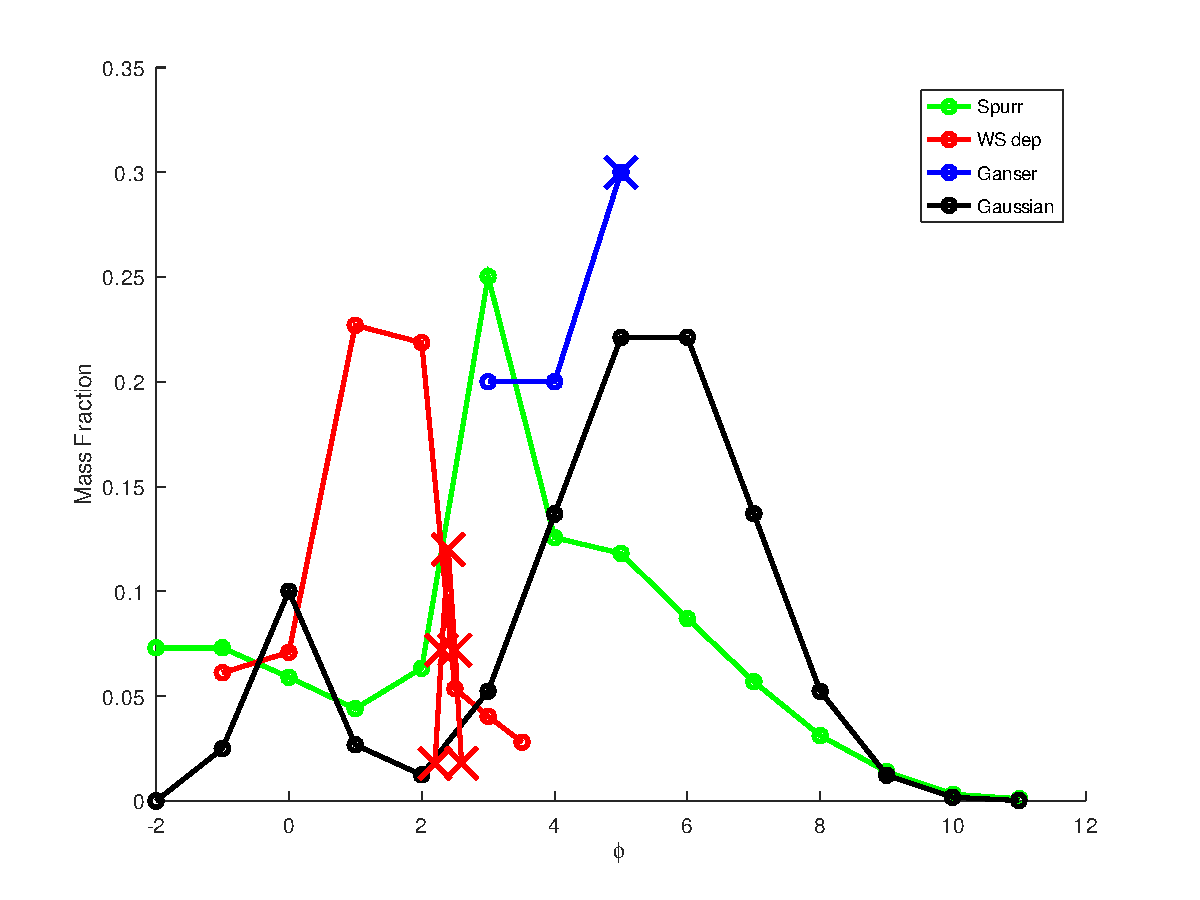
\includegraphics[angle=0,scale=0.7]{Figures/Scripts/InputGSD/FigInputGSD.pdf}
\parbox{15cm}{\caption{\label{FigInputGSD}
Example grain-size distributions. The secondary populations (aggregates for the web
server deposit simulations and the flakes for the Ganser model) are shown with
crosses}}
\end{center}
\end{figure}

\paragraph{Block 8}: Locations of vertical profiles\\
In some cases it has been useful to plot vertical profiles through the ash cloud, as for
example, when ground-based LiDAR data were available over Europe during the 2010
eruption of Eyjafjallaj\"okull. In that case, the lines in Block 8 appeared as follows:

The first line contains an integer indicating the number of locations
(\texttt{nlocs}) where
vertical profiles are to be recorded. If \texttt{nlocs}=0 (as in the example input file), no
lines follow in this block. Otherwise, \texttt{nlocs} lines follow, giving the locations for
each profile in the coordinate system appropriate for this model run (in this case,
degrees longitude and latitude, respectively), followed by an optional station name.
Upon execution, Ash3d writes out text files with the names v\texttt{vprofile0001.txt},
\texttt{vprofile0002.txt}, \texttt{vprofile0003.txt}, \texttt{vprofile0004.txt},
containing vertical profiles at each
of these locations. Below is a truncated illustration of the output contained in
\texttt{vprofile0001.txt}:

The header gives the x and y
coordinates of this location. The numbers in the first row of the table,
``0.250'', ``0.750'', ``1.250'', etc., are the elevations (km) of each cell center in the
model. Each row of data following contains the date and time (UTC, in yyyymmddhh.hh),
the number of hours after the beginning of the eruption, and the concentrations
($\mathrm{mg \, m^-3}$) of tephra at each elevation.
Ash3d writes out a line of output every 10 time
steps as long as the cloud is passing overhead.

\paragraph{Block 9}: Comment lines\\
Line 1 of this block gives the name of the output file containing the 3-D cloud
structure, if this output is specified in Line 15 of Block 4.
Line 2 gives the title of the simulation. If the 3-D cloud structure is written
out to a NetCDF file (as specified in Line 16 of Block 4), this title is included
in that file.
Line 3 gives an optional comment that may be written out to the same NetCDF file.

\subsection{Extensions to the control file: Optional Modules}

After these nine required blocks have been read, Ash3d scans the input file to search
for the term ``\texttt{OPTMOD=}". If this is found, then the corresponding optional
module input block is read. This is primarily used in the development of
research branches of the code, but there are a few that are part of the main
code.

\paragraph{\texttt{RESETPARAMS}}
If a block with \texttt{OPTMOD=RESETPARAMS} is found, then a block of the input
file is read that allows the user to reset the default value of several global
variables. For example, the following block would reset the default magma
density and deposit density.
\small
\begin{verbatim}
***********************
# Reset parameters
***********************
OPTMOD=RESETPARAMS
 MagmaDensity   = 3500.0
 DepositDensity = 1300.0
*******************************************************************************
\end{verbatim}
\normalsize

The full list of parameters that can be reset are given in Table \ref{tab:ResetParam}.
\small
\begin{table}[htbp]
\begin{center}
\begin{tabular}{| l | l | l | l |}
\hline
\texttt{name} & Default value & Units & Description \\
\hline
\texttt{MagmaDensity}      & 2500.0   & $\mathrm{kg/m^3}$  &  Density for DRE calculations \\
\texttt{DepositDensity}    & 1000.0   & $\mathrm{kg/m^3}$  &  Density of tephra deposit \\
\texttt{LAM\_GS\_THRESH}   & 250.0    & $\mathrm{m}$/      &  mean free path for Cunningham slip \\
\texttt{AIRBORNE\_THRESH}  & 1.0e-3   & $\mathrm{kg}$      &  Tot. Airborne mass threshold for bin skipping \\
\texttt{GRAV}              & 9.81     & $\mathrm{m/s^2}$   &  Gravitational acceleration \\
\texttt{RAD\_EARTH}        & 6371.229 & $\mathrm{km}$      &  Radius of Earth \\
\texttt{CFL}               & 0.80     & unitless           &  Courant-Friedrichs-Lewy constant \\
\texttt{DT\_MIN}           & 1.0e-5   & $\mathrm{hour}$    &  Minimum allowed time-step \\
\texttt{DT\_MAX}           & 1.0      & $\mathrm{hour}$    &  Maximum allowed time-step \\
\texttt{ZPADDING}          & 1.3      & unitless           &  Scaling factor for height of z-grid \\
\texttt{ZSCALING\_ID}      & 0        & case ID            &  z-grid case (0=No topo;1=shifted;2=scaled) \\
\texttt{DEPO\_THRESH}      & 1.0e-1   & $\mathrm{mm}$      &  Threshold value to output deposit \\
\texttt{DEPRATE\_THRESH}   & 1.0e-2   & $\mathrm{mm/hour}$ &  Threshold value to output deposit rate \\
\texttt{CLOUDCON\_THRESH}  & 1.0e-3   & $\mathrm{t/km^3}$  &  Threshold value to output cloud concentration \\
\texttt{CLOUDCON\_GRID\_THRESH}&1.0e-7& $\mathrm{t/km^3}$  &  Threshold value for \texttt{FAST\_SUBGRID} \\
\texttt{CLOUDLOAD\_THRESH} & 1.0e-2   & $\mathrm{t/km^2}$  &  Threshold value to output cloud load \\
\texttt{THICKNESS\_THRESH} & 1.0e-3   & $\mathrm{mm}$      &  Threshold value to output deposit \\
\texttt{StopValue\_FracAshDep} & 0.99 & unitless           &  Stop condition for fraction deposited \\
\texttt{DBZ\_THRESH}       & -2.0e+1  & $\mathrm{dB}$      &  Threshold value to output radar reflectivity \\
\texttt{VelMod\_umb}       & 1        & case ID            &  Umbrella velocity model: 1 \cite{Costa14} or 2 \cite{Webster20} \\
\texttt{lambda\_umb}       & 0.2      & unitless           &  Suzuki constant for umbrella cloud \\
\texttt{N\_BV\_umb}        & 0.02     & $\mathrm{s^{-1}}$  &  Brunt-Va\"isala frequency for umbrella cloud \\
\texttt{k\_entrainment\_umb} & 0.1    & unitless           &  Entrainment coefficient for umbrella cloud \\
\texttt{SuzK\_umb}         & 12.0     & unitless           &  Suzuki parameter for umbrella cloud \\
\texttt{useMoistureVars}   & 0        & logical            &  0/1=F/T use RelHum and SpecHum \\
\texttt{useVz\_rhoG}       & 1        & logical            &  0/1=F/T Vz=FinDif v.s. Vz=rho.grav \\
\texttt{useWindVars}       & 0        & logical            &  0/1=F/T include vel in output \\
\texttt{useOutprodVars}    & 1        & logical            &  0/1=F/T include 2-D products in output \\
\texttt{useRestartVars}    & 0        & logical            &  0/1=F/T include ashcon in output \\
\texttt{cdf\_institution}  & USGS     & text               &  Institution name \\
\texttt{cdf\_run\_class}   & Analysis & text               &  Analysis, Hypothetical, Forecast \\
\texttt{cdf\_url}          & url      & text               &  Reference web page \\
\hline
\end{tabular}
\caption{\label{tab:ResetParam}Parameters that can be reset through \texttt{OPTMOD=RESETPARAMS}}
\end{center}
\end{table}
\normalsize

\subsection{Environment variables}
Some variables can be set at run-time through the use of environment variables on a Unix
system. These are not needed, but can be used to change the default values if desired.
There are four environment variables that Ash3d will test at run-time:


\paragraph{\texttt{ASH3DHOME}:}
If the Ash3d executable was compiled to read the
airport and volcano database files at
run-time, the path to these external files should be set when compiled. The default is
\texttt{/opt/USGS/Ash3d}, but this is set in the \texttt{makefile} by the \texttt{INSTALLDIR}
variable. If the files were subsequently moved, or if different versions were needed,
Ash3d tests for the environment variable 

\paragraph{\texttt{ASH3DCFL}:} The CFL factor
is set by default to 0.8, but can be overwritten by the environment variable \texttt{ASH3DCFL}.
Note that this factor could be subsequently reset if the optional input block

\paragraph{\texttt{ASH3DVERB}:} When Ash3d is executing, it will write to standard output
various notes about what it is doing, how it has interpreted the control file, information
on the state of the run and progress as well as any closing notes. These notes are mirrored
to a log file (\texttt{Ash3d.lst}). The user has some control over how verbose this output
is by setting the verbosity environment variable \texttt{ASH3DVERB}. There are ten output
levels with lower numbers indicating more messages to standard output. Levels are described
in Table \ref{tab:VerbosityLevels}. The default level is 3. This can be over-ridden, if
for example, there is an error and you would like further information about the position in
the code causing the error, but running:

\texttt{ASH3DVERB=2 ./Ash3d control.inp}

Similarly, if you are running many Ash3d instances and do not want anything written to the
screen, but do want the individual log files, you can use:

\texttt{ASH3DVERB=9 ./Ash3d control.inp}

Level 10 suppresses all output.

\small
\begin{table}[htbp]
\begin{center}
\begin{tabular}{| c | l | l |}
\hline
level & label & Description \\
\hline
1& debug2      & Additional debugging information only written to stdout\\
2& debug1      & Debugging information only written to stdout\\
3& log         & Time step information (this is the limit for writing to logfile)\\
4& info        & Additional information on run set up and shutdown\\
5& statistics  & Details on health of run (timing, mass conservation)\\
6& production  & Major program flow info\\
7& essential   & Only start up and shutdown messages\\
8& error       & No logging to stdout, only stderr (and logfile)\\
9& silent      & No logging to stdout,stderr. Logfile written as normal\\
10& dark       & No logging to stdout,stderr or logfile\\
\hline
\end{tabular}
\caption{\label{tab:VerbosityLevels}Ash3d verbosity levels}
\end{center}
\end{table}
\normalsize

\paragraph{\texttt{ASH3DPLOT}:}
The post-processing utility, \texttt{Ash3d\_PostProc} (described below in
Section \ref{ChapUsageSecPostProc}) can use several graphics packages for
plotting maps and figures. There is a preference hierarchy built in to the
code, based on output type (map, shapefile, vertical transect) as well as
availability on the system. These can be over-ridden by setting the
environment variable \texttt{ASH3DPLOT}=1-4, where 1 corresponds to DISLIN,
2 PLplot, 3 gnuplot, and 4 GMT. For example, the default contouring package
for building shapefiles is gnuplot, but DISLIN can be used via:

\texttt{ASH3DPLOT=1 ./Ash3d\_PostProc 3d\_tephra\_fall.nc 5 5}

\paragraph{\texttt{OMP\_NUM\_THREADS}:}
If Ash3d was compiled with OpenMP, then the number of threads available
at run-time can be adjusted with this environment variable.

\texttt{OMP\_NUM\_THREADS=4 ./Ash3d control.inp}

%\subsection{Help}


\subsection{Executing Ash3d}
To run Ash3d, simply type \texttt{Ash3d} if the executable is in your path, or
the full path to the executable (e.g. \texttt{/opt/USGS/Ash3d/bin/Ash3d}. This
with start an interactive session where the user is prompted for control file.
Next, the user will be prompted whether or not to load a concentration file.
Normally, this is not needed and the user can enter \texttt{no} to continue
with the Ash3d simulation. If \texttt{yes} is entered,
this will allow users to continue a simulation that was aborted or ended prematurely.

\begin{verbatim}
[user@ash3d MtStHelens]$ ./Ash3d 
 Enter name of ESP input file:
MSH.inp
 Load concentration file?
yes
 Enter name of concentration file
3d_tephra_fall.nc
   Step :  time
           1  0.250000000    
           2  0.750000000    
           3   1.25000000    
           4   1.75000000    
           5   2.25000000    
           6   2.75000000    
 Enter timestep for initialization
5
\end{verbatim}

To run Ash3d non-interactively, simply provide the name of the control file as
a command-line argument. This will begin the execution with messages and program
progress written to standard output. All informational messages as well as
error messages are mirrored to a log file (\texttt{Ash3d.lst}). As noted above,
the verbosity of these messages can be adjusted with the environment variable
\texttt{ASH3DVERB}. Also written during execution is the file \texttt{progress.txt},
which contains the fractional progress of the time stepping from start to the maximum
anticipated time step. Simulations might complete prior to reaching 1.0 for a
variety of reasons (all ash has deposited, anticipated number of time steps is
greater than necessary, etc.).

In the initial stage of execution, Ash3d evaluates the control file, checks for
any error in the computational grid layout, grain-size specification, etc.x. It
also evaluates the files specifying the atmospheric conditions and checks for
consistency with the computational grid and requested times. Ash3d then
proceeds with the time integration of Equation \ref{EqGovEqVect}. Stop conditions
are evaluated each time step including: erupted mass has deposited ($<1\%$ remaining aloft),
time exceeds allotted time, all individual grain sizes have been flagged as deposited.
Additional error checks are evaluated such as mass conservation errors greater than
$0.001$ or for any negative tephra volumes (volume aloft, deposited outflow, source).
When a stop condition is met, finalizes output files and terminates.
%
%%%%%%%%%%%%%%%%%%%%%%%%%%%%%%%%%%%%%%%%%%%%%%%%%%%%%%%%%%%%
\section{Post-processing}\label{ChapUsageSecPostProc}
There are many output files that Ash3d can generate as it is running; including
ESRI ASCII files of the deposit accumulation, final deposit thickness, deposit
arrival time, various
measures of the airborne ash cloud (height, cloud load, maximum cloud concentration,
cloud arrival time).  These ASCII files can be loaded into GIS software such
as Arc View or QGIS. Additionally, Ash3d can directly write KML files for each of
the variable listed above which can be viewed interactively with virtual globe
software such as Google Earth. Whether or not to write this output files is specified
in Block 4 of the control file used for the Ash3d simulation. An example of a KML
file for a final deposit is shown in Figure \ref{FigAsh3dOutputKMLDep}.

\begin{figure}[htbp]
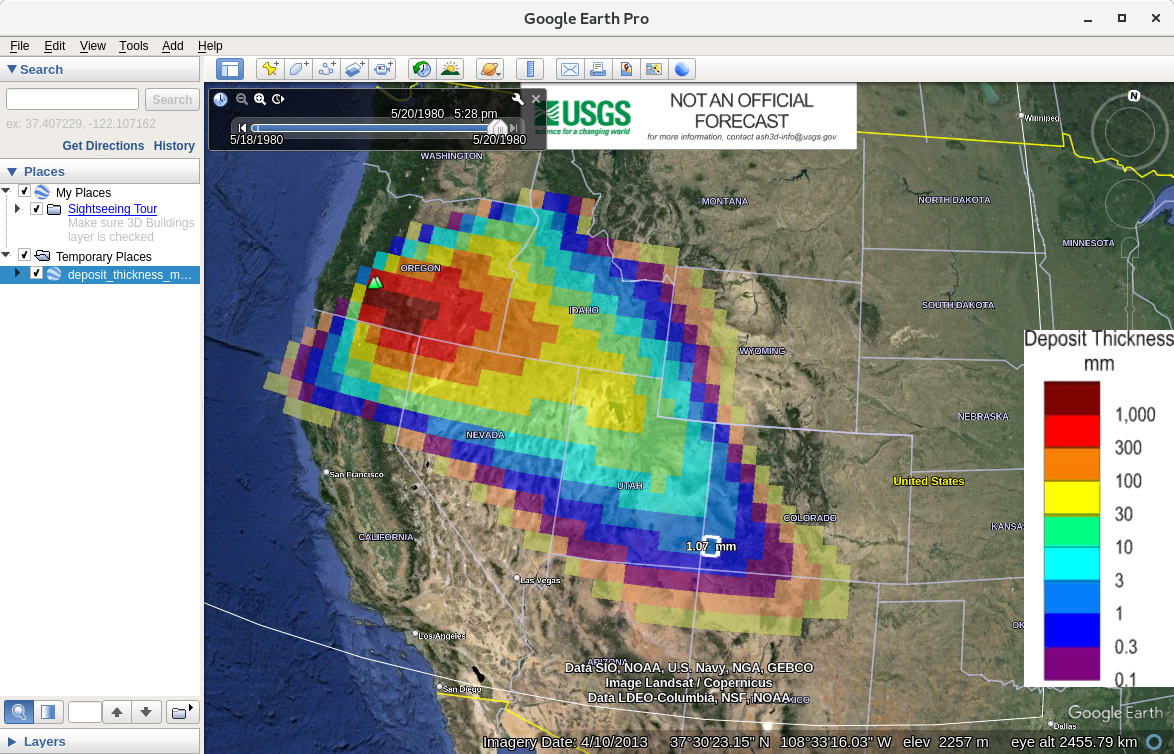
\includegraphics[angle=0,scale=0.35]{Figures/Ash3dOutput_KMLDep_GoogleEarth.png}
\parbox{15cm}{\caption{\label{FigAsh3dOutputKMLDep}
Viewing deposit KML output with Google-Earth}}
\end{figure}

In the KML files, the domain of the Ash3d simulation is outlined with a white line
and the cells are colored according to the cell-average value. The spatial resolution of
the simulation is apparent, as there is no interpolation. Values of individual cells
can be seen simply by mousing over the cell. KML files of deposit variables have cells
clipped to the ground surface.  Cloud variables are pinned to cloud height.

To view the ESRI ASCII files in GIS software, the files can be added as a raster layer
on top of a basemap. The data might need to be shifted to the same periodic mapping
of longitude.  For example, the ASCII cloud height data for the example in Figure \ref{FigAsh3dOutputKMLDep}
has the following header:
\small
\begin{verbatim}
NCOLS    76
NROWS    40
XLLCORNER         225.000
YLLCORNER          33.000
CELLSIZE           0.500          0.500
\end{verbatim}
\normalsize
indicating a lower-left corner at a longitude of $225^{\circ} \, \mathrm{E}$.
The world coastline data has a range of $-180 \rightarrow 180$. The raster data must
be shifted either within the viewing software or by editing the longitude. Figure
\ref{FigAsh3dOutputQgisCH} shows an example of Cloud Height viewed with QGIS.
\begin{figure}[htbp]
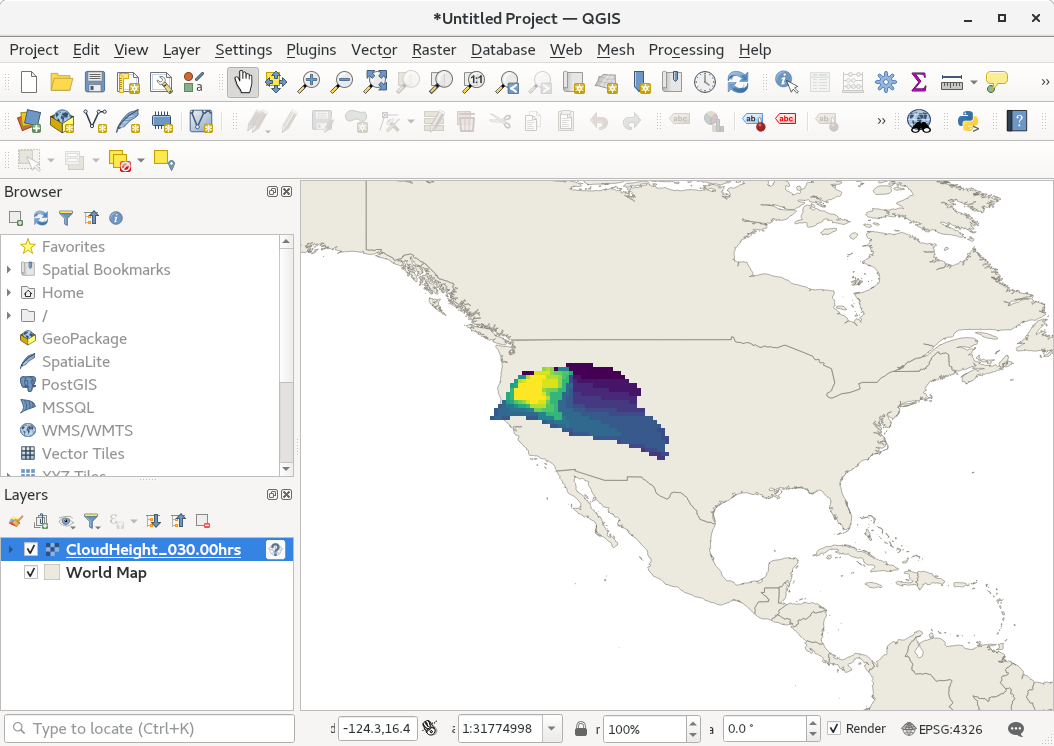
\includegraphics[angle=0,scale=0.35]{Figures/Ash3dOutput_ESRICloudHeight_QGIS.png}
\parbox{15cm}{\caption{\label{FigAsh3dOutputQgisCH}
Viewing cloud height output with QGIS}}
\end{figure}

Other output products written at run-time include text or KML files of ash arrival
time at airports or
points-of-interest (POI) as specified in Block 6 of the control file.
This can also be viewed in Google Earth with the data appearing as white dots for locations
that had ashfall and red dots for points only effected by the drifting cloud. Clicking on
these points will open a descriptive window that gives the time of arrival of the cloud
as well as duration.  If the point is effected by ashfall, a time-series plot will be
included showing the accumulation of the deposit at the site. These plots are generated
by executing \texttt{gnuplot} as a system call within Ash3d, then executing \texttt{gzip}
to bundle the KML file with the linked deposit plots into a compressed KMZ file. This
information is summarized in the file \texttt{ash\_arrivaltimes\_airports.txt}
(Figure \ref{FigAshArrivTimeFormat}).

\begin{figure}[htbp]
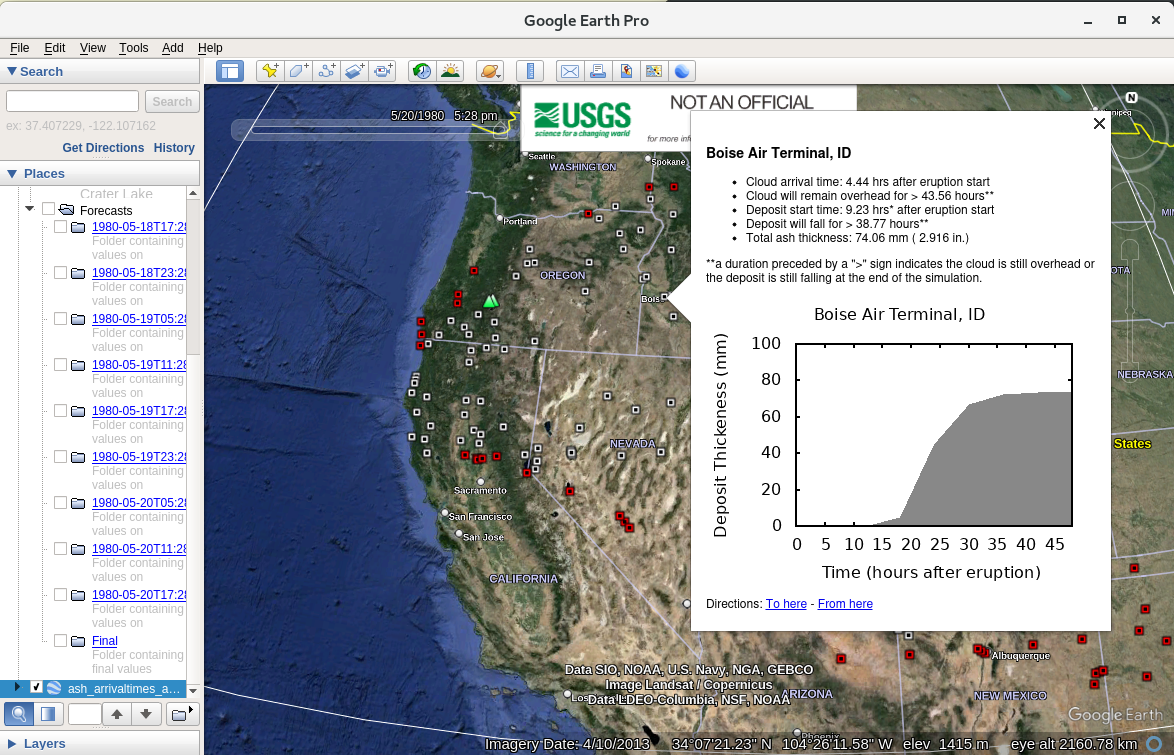
\includegraphics[angle=0,scale=0.35]{Figures/Ash3dOutput_KMLPOIarrival_GoogleEarth.png}
\parbox{15cm}{\caption{\label{FigAsh3dOutputKMLPOIarrivalTS}
Viewing Airport arrival time KML output with Google-Earth}}
\end{figure}

Vertical profiles can be written in ASCII format, if requested in Block 8 and will typically
require post-processing for visualization.

The most general and complete output is the 3-D ash concentration that can be requested on
Line 15 of Block 4 of the control file. If \texttt{ASCII} is selected on Line 16, then
a 3-D ESRI ASCII file of the total ash concentration is written which can be loaded into
a GIS program (e.g. ArcView or QGIS). If \texttt{binary} is specified, then a binary
ash concentration file can be read into a more general visualization software such
as ParaView. The recommended output format is \texttt{netcdf}. If this is selected,
the full ash concentration data ($q(x,y,z,gs,t)$) and full deposit-concentration data is saved at
the requested time steps. Additionally, all the derived variables listed above, such
as deposit thickness, cloud height, arrival times, etc. are included. If Airport/POI
data are requested in Block 4, then these data are also included in the NetCDF output
file on the time steps requested in Block 4.  If vertical profile data are requested in
Block 8, then these data are also stored in the NetCDF file on the time-raster of that
dataset (native time steps of the computation).

In addition to the ash concentration and derived variables listed above, all the
information from the control file is included either as additional variables (grain-size
values or eruptive pulse values) or as global attributes such as the values used for
all resettable parameters, git commit IDs for Ash3d and MetReader, etc.  This enables
a complete reconstruction of the simulation from the information in the NetCDF file.
Since this is such a convenient format and since the full ash concentration data needed
for restarting simulations is seldom needed, cloud and deposit concentration variables
can be suppressed if the optional second term on Line 15 of Block 4 is set to 2 (default
is 1, indicating to write out restart concentrations).

\small
\begin{verbatim}
yes 2   #Write out 3-D ash concentration at specified times?                       
\end{verbatim}
\normalsize

To simply inspect the output, the NetCDF file is COARDS-compliant (naming
convention for dimensions) and can be directly read by many visualization
programs (e.g. ncview, shown in Figure \ref{FigAsh3dOutputncview}).
\begin{figure}[htbp]
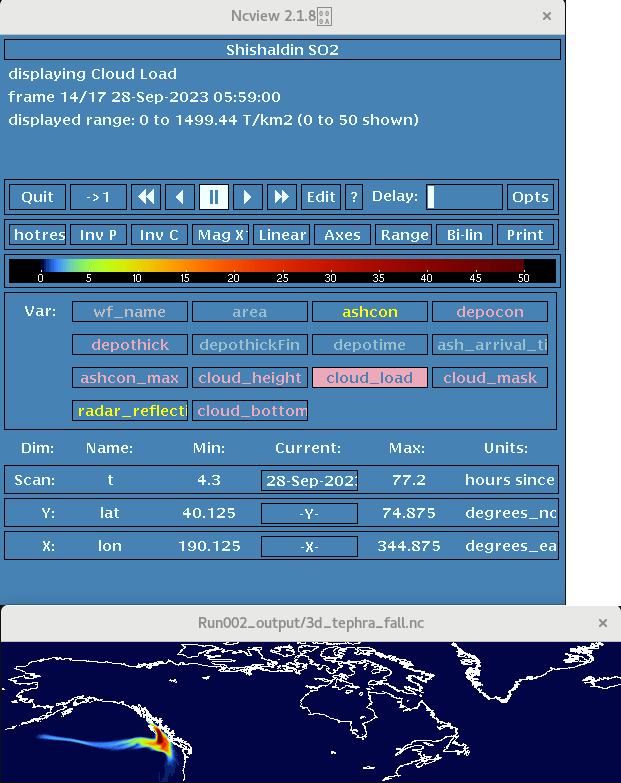
\includegraphics[angle=0,scale=0.5]{Figures/Ash3d_Viz_ncview.png}
\parbox{15cm}{\caption{\label{FigAsh3dOutputncview}
Displaying NetCDF file using general data viewer}}
\end{figure}
These programs display the data over a map and allow an easy visualization
of the evolution of the cloud or deposit.

\subsection{\texttt{Ash3d\_PostProc}}\label{ChapUsageSecPostProc_tool}
The Ash3d repository includes a post-processing tool (\texttt{Ash3d\_PostProc})
that can be used to generate simple maps from the NetCDF output file.
Any of the standard output products (ESRI ASCII, KML/KMZ, binary) can
be recreated using this tool along with png images of 2-D data in mapview
(or contour plots for vertical profiles) or shapefiles of 2-D data. To
produce image files, \texttt{Ash3d\_PostProc} can use a variety of geographic
plotting software. Both DISLIN and PLplot are available as libraries and can
be linked to \texttt{Ash3d\_PostProc} at compilation time. DISLIN includes
the feature where contour data can be accessed by \texttt{Ash3d\_PostProc}
and used to generate shapefiles. This is the preferred means of generating
shapefiles on a Microsoft Windows system. \texttt{Ash3d\_PostProc} can also
generate maps using \texttt{gnuplot} and Generic Mapping Tools (GMT) via
the writing and execution of temporary scripts.

\texttt{Ash3d\_PostProc} is designed to be a quick tool for converting the
NetCDF output of an Ash3d run to format that can be visualized. This tool
can be run interactively by just running the executable with no command-line
arguments. If one argument is provided, it is interpreted to be the name of a
control file (described below). Minimal instructions for running this tool
are available by running the program with a -h as the only argument
\small
\begin{verbatim}
[user@ash3d example_problem]$ ./Ash3d_PostProc -h
 Dislin   T
 Plplot   T
 Gnuplot  T
 GMT      T
                                                                                
 Ash3d post-processing tool: Ash3d_PostProc                                     
                                                                                
Usage: Ash3d_PostProc control_file [t_index]                                    
           or                                                                   
       Ash3d_PostProc infile output_product format                              
  where: infile   = the NetCDF file written by Ash3d                            
   output_product = 1 full concentration array                                  
                    2 deposit granularity                                       
                    3 deposit thickness (mm time-series)                        
                    4 deposit thickness (inches time-series)                    
                    5 deposit thickness (mm final)                              
                    6 deposit thickness (inches final)                          
                    7 ashfall arrival time (hours)                              
                    8 ashfall arrival at airports/POI (mm)                      
                    9 ash-cloud concentration (mg/m3)                           
                   10 ash-cloud height (km)                                     
                   11 ash-cloud bottom (km)                                     
                   12 ash-cloud load (T/km2 or )                                
                   13 ash-cloud radar reflectivity (dBz)                        
                   14 ash-cloud arrival time (hours)                            
                   15 topography                                                
                   16 profile plots                                             
           format = 1 ASCII/ArcGIS                                              
                    2 KML/KMZ                                                   
                    3 image/png                                                 
                    4 binary                                                    
                    5 shape file                                                
         [t_index] = index of time slice to plot; -1 for final (optional)
\end{verbatim}
\normalsize
For example, to generate a contour plot of the final deposit thickness in $\mathrm{mm}$
from the output NetCDF file, enter:
\small
\begin{verbatim}
Ash3d_PostProc 3d_tephra_fall.nc 5 3
\end{verbatim}
\normalsize

The preferred graphics package is set at the time of compilation depending on the
system (Linux, Windows, MacOS) and the availability of the libraries. These can
always be overwitten at run-time with the environment variable \texttt{ASH3DPLOT},
where: 1=DISLIN, 2=PLplot, 3=gnuplot, and 4=GMT. Examples of these plotting packages
is shown in Figure \ref{FigAsh3dAsh3dPP_map2x2}.

\small
\begin{verbatim}
ASH3DPLOT=3 Ash3d_PostProc 3d_tephra_fall.nc 5 3
\end{verbatim}
\normalsize

\begin{figure}[htbp]
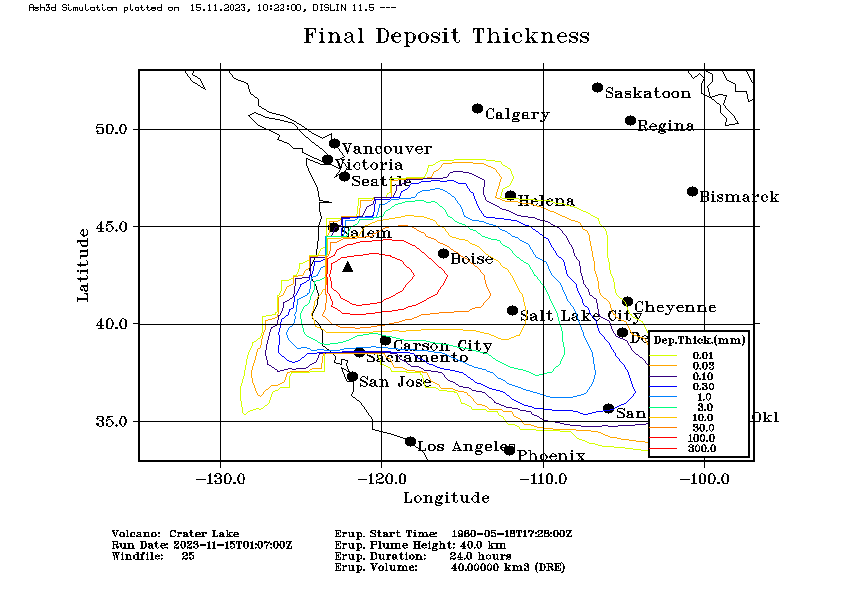
\includegraphics[angle=0,scale=0.25]{Figures/Ash3d_Deposit____final_dislin.png}
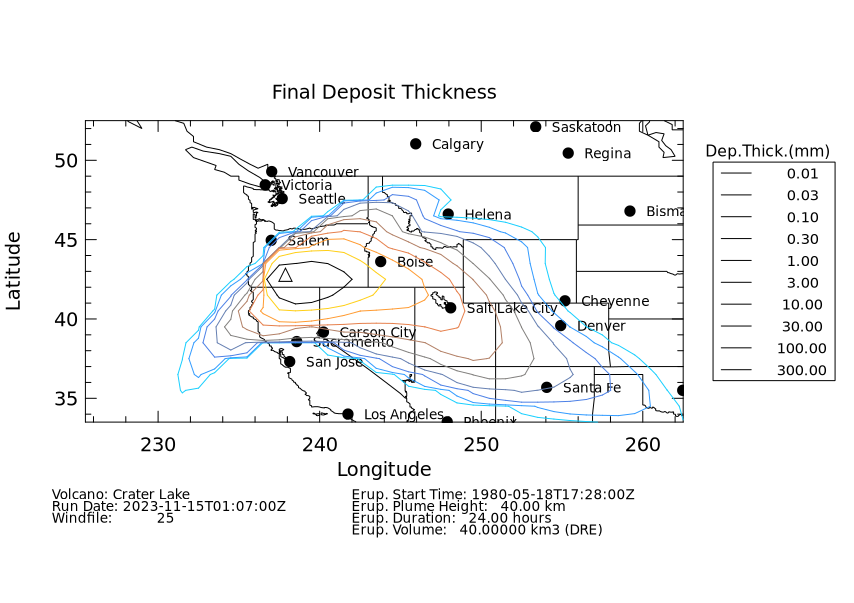
\includegraphics[angle=0,scale=0.25]{Figures/Ash3d_Deposit____final_plplot.png}
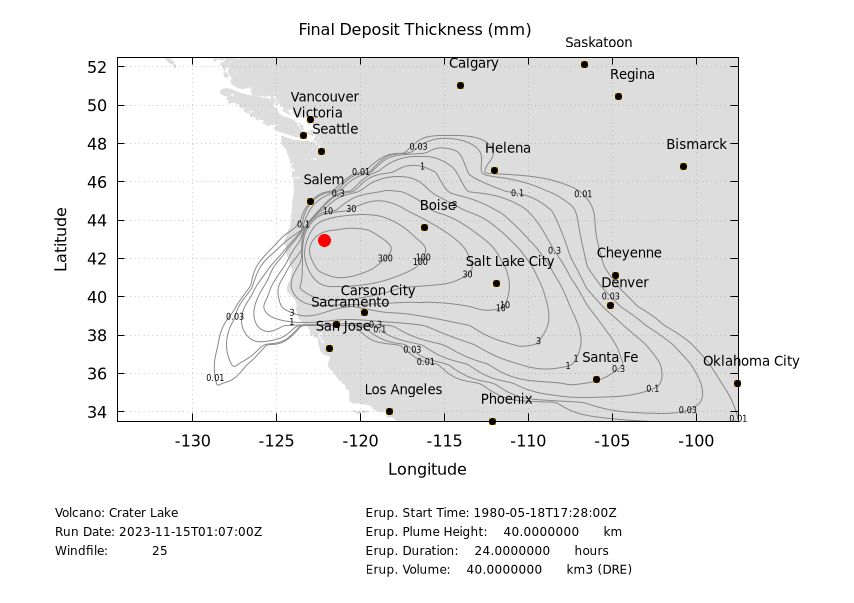
\includegraphics[angle=0,scale=0.25]{Figures/Ash3d_Deposit____final_gnuplot.png}
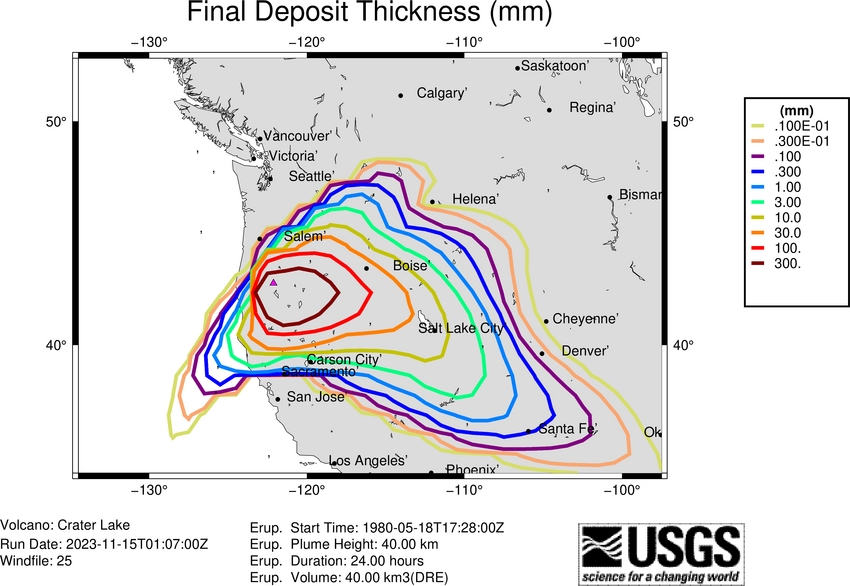
\includegraphics[angle=0,scale=1.0]{Figures/Ash3d_Deposit____final_gmt.png}
\parbox{15cm}{\caption{\label{FigAsh3dAsh3dPP_map2x2}
Final deposit contour maps using \texttt{Ash3d\_PostProc} with different plotting packages.}}
\end{figure}

To generate a shapefile of the cloud load at step 3 of the output file, enter:
\small
\begin{verbatim}
Ash3d_PostProc 3d_tephra_fall.nc 12 5 3
\end{verbatim}
\normalsize

This will create four files: \texttt{AshCdLod.shx}, \texttt{AshCdLod.shp},
\texttt{AshCdLod.prj}, \texttt{AshCdLod.dbf}, which are then bundled into
\texttt{AshCdLod.zip} using a system call to \texttt{gzip}. This shapefile
can then be loaded as vector layer in a GIS program. Figure \ref{FigAsh3dAsh3dPP_shape} shows
the shapefile generated above using QGIS and Figure \ref{FigAsh3dAsh3dPP_shapeAtr} shows the
shapefile attributes.

\begin{figure}[htbp]
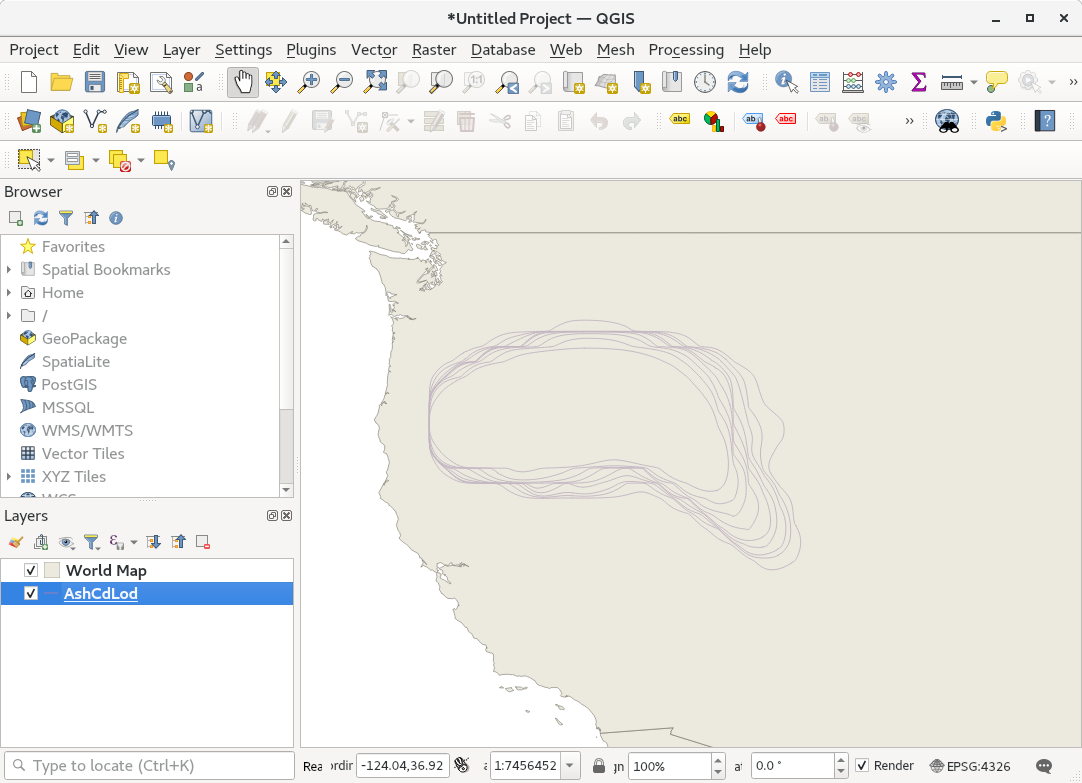
\includegraphics[angle=0,scale=0.35]{Figures/Ash3dOutput_ShpCloudLoad_QGIS.png}
\parbox{15cm}{\caption{\label{FigAsh3dAsh3dPP_shape}
Shapefile of cloud load added as a vector layer in QGIS.}}
\end{figure}

\begin{figure}[htbp]
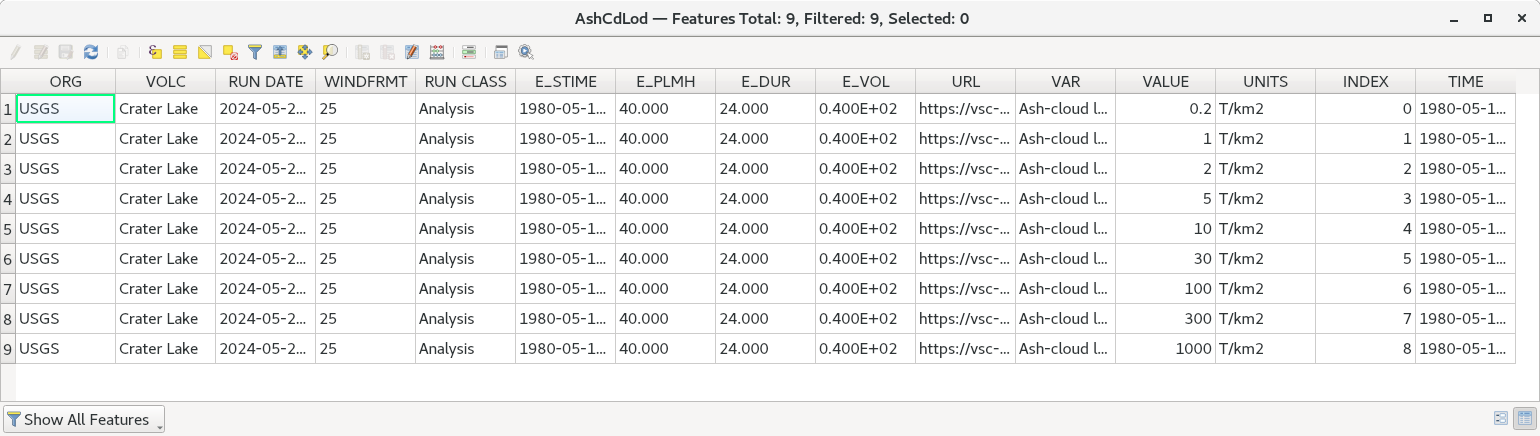
\includegraphics[angle=0,scale=0.27]{Figures/Ash3dOutput_ShpAtrCloudLoad_QGIS.png}
\parbox{15cm}{\caption{\label{FigAsh3dAsh3dPP_shapeAtr}
Shapefile of cloud load shapefile.}}
\end{figure}

In the attribute table shown in Figure \ref{FigAsh3dAsh3dPP_shapeAtr}, the fields for
ORG, RUN CLASS and URL are the default values, but these can be changed in the
optional \texttt{RESETPARAMS} block of the control file.

\small
\begin{verbatim}
***********************
# Reset parameters
***********************
OPTMOD=RESETPARAMS
 cdf_institution      = Volcano Observatory
 cdf_run_class        = Forecast
 cdf_url              = https://volcano-observatory/model-forecasts
*******************************************************************************
\end{verbatim}
\normalsize

\texttt{Ash3d\_PostProc} is a convenient tool for plotting the vertical profiles.
To plot profiles using the gnuplot graphics package, run:
\small
\begin{verbatim}
ASH3DPLOT=3 ./Ash3d_PostProc 3d_tephra_fall.nc 16 3
\end{verbatim}
\normalsize
which in this case will generate two files for the two requested profile locations:
\texttt{gnupl\_0001.png} and \texttt{gnupl\_0002.png}. Profile 2 is shown in Figur
\ref{}.

\begin{figure}[htbp]
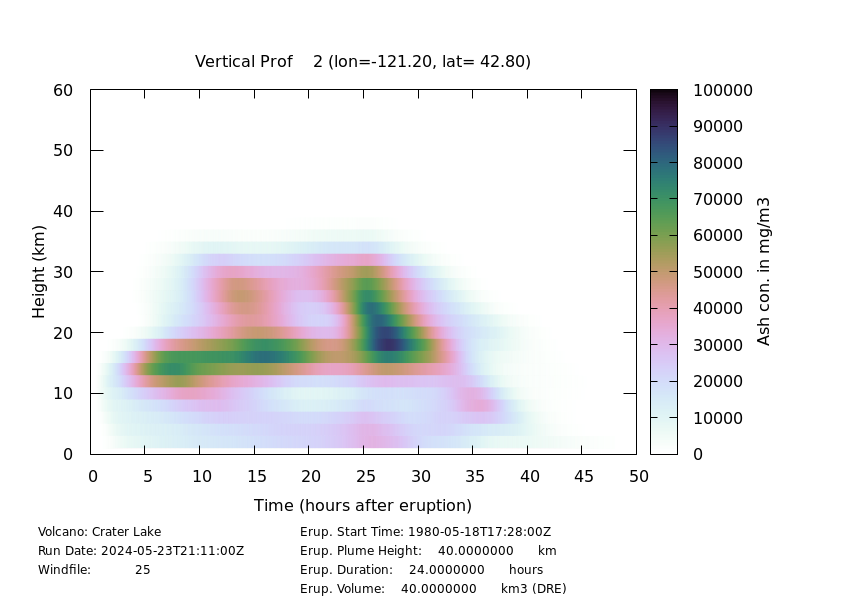
\includegraphics[angle=0,scale=0.5]{Figures/gnupl_0002.png}
\parbox{15cm}{\caption{\label{FigAsh3dAsh3dPP_vertprof}
Vertical profile of ash concentration at location 2.}}
\end{figure}

Using \texttt{Ash3d\_PostProc} with command-line arguments is meant to be a
quick tool for generating plots from the NetCDF output file. Using a control
file, however, allows much more flexibility and allows plotting maps
from 2-D ASCII or binary files, or to customize the contour levels and colors.

Below is an example of a control file that can be used to convert a 2-D ESRI ASCII
output file of the deposit thickness to a map image with custom contour levels.

\small
\begin{verbatim}
DepositFile_____final.dat       data_filename
1                       input format code (1=ASCII, 2=binary, 3=NetCDF)
test.inp                Ash3d_control_file_name   (skipped if datafile is NetCDF)
5                       invar [outvar]    input variable and output variable, if different
2 1                     ndims Only needed for format 1 or 2, LatLonFlag
38 20                   nx ny [nz] Also only needed for format 1 or 2
1.0 1.0                 dx dy [dz] Needed if not a part of the data file
225.0 33.0              srtx srty         Start x and y
3                       output format     (1=ASCII, 2=KML 3=image, 4=binary, 5=shapefile)
4                       plot_pref         (1=dislin, 2=plplot, 3=gnuplot, 4=GMT)
-1                      time_step         Only needed if input file is multi-timestep (eg NetCDF) (-1 for final, -2 for all)
0                       Filled contour flag (1 for filled, 0 for lines)
1 5                     custom contour flag (1 for true, 0 for false), number of contours
1.0 3.0 10.0 50.0 100.0 lev(ncont)  : contour levels
100 100 100 100 255     R(ncont)    : Red channel of RGB
100 150 200 150   0     G(ncont)    : Green channel of RGB
200 150 100  50   0     B(ncont)    : Blue channel of RGB
\end{verbatim}
\normalsize

Line 1 contains the data file name, in this case
\texttt{DepositFile\_\_\_\_\_final.dat}, but it could be
the output NetCDF file or any 2/3-D binary or ASCII output file.
Line 2 specifies the format code for ASCII, binary or NetCDF.
Line 3 is the name of the Ash3d control file for this run. This is needed to know the geometry
of the simulation, the time steps, volcano name, eruption source parameters, and
other information needed for annotating the maps or other output products. If the
input data file is the Ash3d NetCDF output file, then this Ash3d input control file
is ignored as all the information required is stored in the NetCDF file.
Line 4 is the variable code for the input file, which is assumed to be the output
variable code unless a second code for the output variable is provided. For example, if
the data file is the Ash3d NetCDF data file, then entering `5` in line 4 will result
in a plot of the final deposit thickness. If the input data file is a 3-D binary
file of the airborne ash concentration, but cloud load is needed for the output, line
4 would contain \texttt{1 12}.
Line 5 contains the number of dimensions of the data file (2 or 3) and a code indicating if
the data are projected or in lon/lat coordinates (0 or 1). \texttt{Ash3d\_PostProc} currently
only can plot projected data using GMT.
Line 6 gives the number of nodes in the x,y, and possibly z directions for the data file.
Line 7 gives the grid spacing for all the coordinate directions of the file and line 8
gives the start coordinates.
Line 8 is the output format code where 1=ASCII, 2=KML 3=image, 4=binary, 5=shapefile.
Line 9 is the plotting package preference code: 1=DISLIN, 2=PLplot, 3=gnuplot, 4=GMT.
Line 10 is the time step to plot. -1 can be entered to plot the last time step of the
file.
Line 11 is a flag to indicate if the plot should have contour lines (0) or filled contours (1).
This option is not yet fully functional and only contour lines are available.
Line 12 starts with a flag allowing custom contour levels (1) to override the default
levels for that variable. If this flag is set, a second value is read, giving the
number of custom levels (\texttt{nlev}).
If custom contours are requested, then four additional lines are read in the control file.
Line 13 contains the \texttt{nlev} floating point values for the contour levels in the
default units of the output variable.
Lines 14, 15, and 16 are the \texttt{nlev} integer values of the RGB components of the colors (0-255).

\subsection{Generating maps with GMT}\label{ChapUsageSecPostProcGMT}
There are many programs that can be used for generating maps from Ash3d output. We primarily
use Generic Mapping Tools (GMT) due to its flexibility, customization and ease of use in
bash scripts. Plots generated on the Ash3d web-servers use scripts that read information
about the Ash3d run from the NetCDF file, dynamically plot data, select the top most populous
cities in the domain for annotating, and evaluate legend placement based on deposit location.
These scripts are described in more detail in Chapter \ref{ChapExtraToolExamples}.

There are many tutorials online for learning GMT. Here we just show an example script
that can be used to generate a basemap, display shaded topography and overlay
deposit contours.  The resulting plot is shown in 
\ref{FigAsh3dAsh3d_NevDeRuizGMT}.

\footnotesize
\begin{verbatim}
#!/bin/bash

AREA=-R-80.0/-70.0/2.0/8.0
PROJ=-JM-75.0/4.0/20
BASE=-Ba2g2/2g1

gmt makecpt -Cetopo1 -D -V -T-3500/3500/10 > topo.cpt

gmt grdconvert gebco_2023_n20.0_s-10.0_w-100.0_e-50.0.nc?elevation fulltopo.grd
gmt grdcut fulltopo.grd -Gtopo.grd $AREA
gmt grdgradient topo.grd -Gtopo.grad -A90/20 -fg

gmt pscoast $BASE $AREA $PROJ -Dh -G -K > temp.ps
gmt grdimage topo.grd -Itopo.grad $AREA $PROJ -Ctopo.cpt -K -O >> temp.ps
gmt pscoast -Q $BASE $AREA $PROJ -Dh -K -O >> temp.ps

echo "0.01   C" > dpm_0.01.lev   #deposit (0.01 mm)
echo "0.03   C" > dpm_0.03.lev   #deposit (0.03 mm)
echo "0.1    C"  > dpm_0.1.lev   #deposit (0.1 mm)
echo "0.3    C"  > dpm_0.3.lev   #deposit (0.3 mm)
echo "1.0    C"  >   dpm_1.lev   #deposit (1 mm)
echo "3.0    C"  >   dpm_3.lev   #deposit (3 mm)
echo "10.0   C"  >  dpm_10.lev   #deposit (1 cm)
echo "30.0   C"  >  dpm_30.lev   #deposit (3 cm)
echo "100.0  C"  > dpm_100.lev   #deposit (10cm)
echo "300.0  C"  > dpm_300.lev   #deposit (30cm)

infile="../3d_tephra_fall_ERA5_Topo.nc"
##get volcano longitude, latitude
VCLON=`ncdump -h ${infile} | grep b1l5 | cut -d\" -f2 | awk '{print $1}'`
VCLAT=`ncdump -h ${infile} | grep b1l5 | cut -d\" -f2 | awk '{print $2}'`
dep_grd="dep_fin.grd"
gmt grdconvert "$infile?depothickFin" ${dep_grd}
gmt grdcontour ${dep_grd}   $AREA $PROJ $BASE -Cdpm_0.01.lev -A- -W3,214/222/105   -O -K >> temp.ps
gmt grdcontour ${dep_grd}   $AREA $PROJ $BASE -Cdpm_0.03.lev -A- -W3,249/167/113   -O -K >> temp.ps
gmt grdcontour ${dep_grd}   $AREA $PROJ $BASE -Cdpm_0.1.lev  -A- -W3,128/0/128   -O -K >> temp.ps
gmt grdcontour ${dep_grd}   $AREA $PROJ $BASE -Cdpm_0.3.lev  -A- -W3,0/0/255     -O -K >> temp.ps
gmt grdcontour ${dep_grd}   $AREA $PROJ $BASE -Cdpm_1.lev    -A- -W3,0/128/255   -O -K >> temp.ps
gmt grdcontour ${dep_grd}   $AREA $PROJ $BASE -Cdpm_3.lev    -A- -W3,0/255/128   -O -K >> temp.ps
gmt grdcontour ${dep_grd}   $AREA $PROJ $BASE -Cdpm_10.lev   -A- -W3,195/195/0   -O -K >> temp.ps
gmt grdcontour ${dep_grd}   $AREA $PROJ $BASE -Cdpm_30.lev   -A- -W3,255/128/0   -O -K >> temp.ps
gmt grdcontour ${dep_grd}   $AREA $PROJ $BASE -Cdpm_100.lev  -A- -W3,255/0/0     -O -K >> temp.ps
gmt grdcontour ${dep_grd}   $AREA $PROJ $BASE -Cdpm_300.lev  -A- -W3,128/0/0     -O -K >> temp.ps

# Last gmt command is to plot the volcano and close out the ps file
echo $VCLON $VCLAT '1.0' | gmt psxy $AREA $PROJ -St0.1i -Gblack -Wthinnest -O >> temp.ps

\end{verbatim}
\normalsize


\begin{figure}[htbp]
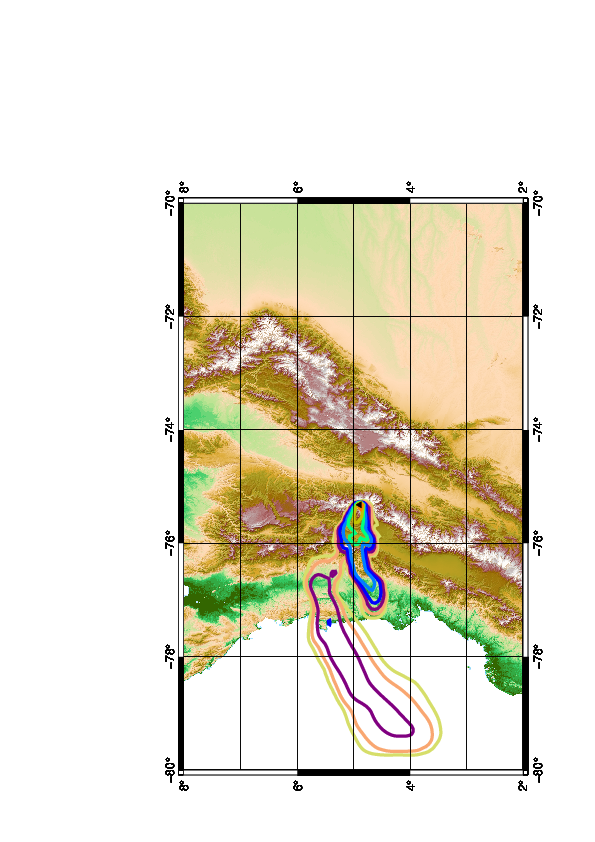
\includegraphics[angle=-90,scale=0.6]{Figures/NevadoDelRuiz89.png}
\parbox{15cm}{\caption{\label{FigAsh3dAsh3d_NevDeRuizGMT}
GMT map of Ash3d deposit for Nevado del Ruiz}}
\end{figure}

%processing ESRI ASCII files with GMT\\
%processing NetCDF files with GMT\\
%scripts from Ash3d\_web\\
%conversion tool\\
%tecplot

%AFWA GUI












